% header ---------------------------------------
\documentclass[a4paper,12pt, titlepage]{article}  % book instead of article. Note: maybe add twosided later
\usepackage{graphicx}
\usepackage[ansinew]{inputenc} % deutsche Umlaute
\usepackage{url}
\usepackage{amsmath}
\usepackage{morefloats}

\newcommand{\cl}{\mathcal{L}}   % cl stands for compressed layer
\newcommand{\oh}{\mathcal{O}}   % big oh notation

% begin the document ---------------------------
\begin{document}

% titlepage -----------------------------------
\begin{titlepage}
	\title{\textbf{An efficient implementation of the optimal paging algorithm}}
	
	\author{
	A thesis submitted for the degree of \\
	\textbf{Bachelor of Computer Science} \\
	\\
	by \\
	\textbf{Edgardo Deza}\\
	\\
	\large Supervisor: \\
	\normalsize Prof. Dr. Ulrich Meyer\\
	\\
	\large Advisers:\\
	\normalsize Dipl.-Inf. Andrei Negoescu\\
	\normalsize Gabriel Moruz, PhD\\
       \\
        \large Reviewers:\\
        \normalsize Prof. Dr. Ulrich Meyer, Prof. Dr. Georg Schnitger\\   %<------  put these double backslashes here!! otherwise the first page is blank
	}
	\date{
	\normalsize Professorship for Algorithm Engineering\\
	\normalsize Institute for Computer Science\\
	\normalsize Goethe-Universit\"at, Frankfurt am Main\\
	
\includegraphics[scale=0.23]{./figures/Goethe-logo.pdf}
	}
\end{titlepage}
% end of titlepage -----------------------------

\pagestyle{empty}
%\pagenumbering{Roman}
\maketitle
%\thispagestyle{empty} % prevents display of page number


%----- EIDESSTATTLICHE ERKLAERUNG
\clearpage
%\subsection*{Eidesstattliche Erkl\"arung}
%Ich erkl\"are hiermit an Eides Statt, dass ich die vorliegende Arbeit
%selbst\"andig und ohne Benutzung anderer als der angegebenen Hilfsmittel
%angefertigt habe; die aus fremden Quellen (einschlie\ss lich elektronischer
%Quellen) direkt oder indirekt \"ubernommenen Gedanken sind ausnahmslos als
%solche kenntlich gemacht.
%\\\\\\
%\noindent Frankfurt, den 
%\begin{flushright}
%$\overline{~~~~~~~~~\mbox{(Edgardo Deza)}~~~~~~~~~}$
%\end{flushright}
% vorlage: http://www.wiso.uni-kiel.de/vwlinstitute/Raff/downloads/aktuelles/Vorlage_TeX.tex

\subsection*{Declaration of authorship}
I hereby declare that this thesis is entirely the result of my own work except where otherwise indicated. 
I have only used the resources given in the list of references.
\\\\\\
\noindent Frankfurt am Main, November 15, 2012
\begin{flushright}
$\overline{~~~~~~~~~\mbox{(Edgardo Deza)}~~~~~~~~~}$
\end{flushright}
% from: http://www.in.tum.de/en/for-students-of-the-tum/master-programs/computational-science-and-engineering/academics/masters-thesis.html
% from: http://upcommons.upc.edu/pfc/bitstream/2099.1/14636/1/MasterThesis-ChristineDoig.pdf



%------ACKNOWLEDGEMENT
\clearpage
\subsection*{Acknowledgement}
I thank Ulrich Meyer for giving me the opportunity to write my thesis on this interesting topic. 
His enthusiasm for algorithm engineering has kindled my interest in online paging.\\
\\
I am grateful to Andrei Negoescu for being my adviser. Without his help and encouragement this thesis
would not have been possible. \\
\\
I thank Gabriel Moruz for his support. He always had an open office door whenever I had a question,
and his expertise proved valuable.\\ 
\\
I wish to thank Georg Schnitger. He immediately accepted my request for being the second reviewer
of my thesis.\\
\\
I am indebted to Diana Firnges. She has often advised me on my study plan.


% abstract ----------------------
%- design and analyzed
%- why, motivation, improvement
%- implemented our new approach, withexperiments
%- application

\begin{abstract}
In this Bachelor thesis we designed a new data structure denoted as LTrees which keeps track of 
the costs that are incurred by the optimal offline paging algorithm OPT~\cite{belady66_opt}. We analyze LTrees and show 
that for a page-set size $m$ it answers the question whether a requested page is in OPT's cache in $\oh(\alpha(2m))$ amortized time, which 
is virtually constant since the inverse Ackermann function $\alpha$ is smaller than 5 for any practical input size.
This presents an improvement over other approaches that require $\oh(\log(m))$~\cite{boyar07} and $\oh(\log(k))$~\cite{brodal11} time, 
where $k$ is the cache size. The space required by LTrees is $\theta(m)$.

Using real-world traces we have examined how LTrees behaves in comparison to a timestamp based 
implementation~\cite{sea12_paper} which we refer to as TStamp. The experiments demonstrate that the runtime 
for LTrees is robust towards different cache sizes, whereas the runtime for TStamp 
can dramatically increase. 

Our data structure can be used as a subroutine for the page replacement algorithm RLRU~\cite{boyar07}. Another application  
is the calculation of the empirical competitive ratio~\cite{moruz_soda12}.

\end{abstract}



%The goal of this Bachelor thesis was to design a data structure which implements the optimal offline paging
%algorithm OPT. Our implementation LTrees consists of linked trees and processes a page request in $\oh(\alpha(2m))$ 
%amortized time, where $m$ is the number of unique pages in the request sequence. The required 
%space is $\theta(m)$. 

%Using real-world traces we have examined how LTrees behaves in comparison to TStamp 
%which is a timestamp based implementation of OPT. The experiments show that the runtime 
%for LTrees is robust towards different cache sizes, whereas the runtime for TStamp 
%can dramatically increase. 

%The goal of this bachelor thesis was to implement the optimal offline paging algorithm. 
%Our implementation LTrees, which stands for Linked Trees, processes a page request in $\mathcal{O}(\alpha(2m))$ amortized runtime and requires 
%$\theta(m)$ space, where $m$ is the number of unique pages in the request sequence and $\alpha$ the inverse Ackermann function.
%For all practical input sizes $n$ the function $\alpha(n)$ is smaller than 5 making the amortized runtime for a page request 
%effectively constant. 
%Moreover, the runtime is independent of the cache size $k$ such that it is robust towards changes in $k$.
% end of abstract -------------------------------------------------


\clearpage
% table of contents

\tableofcontents
\newpage

\pagestyle{plain}
\setcounter{page}{1} % sets the page number to 1


% 1 Introduction -----------------------------------
\section{Introduction}

% 1.1 Memory Hierarchy and paging
\subsection{Memory hierarchy and paging}
We consider a two-level memory hierarchy that consists of a fast but small memory and a slow but large memory.
An example for this can be found in a personal computer: on the one hand the RAM is fast compared to the hard disk, 
on the other hand the size of the RAM is much smaller than that of the hard disk~\cite{memory_hierarchy}. 
The reason why the hard disk is slow is because it is also a mechanical device. 
It consists of a head that is moved by an actuator arm and a rotating disk similar to a record player. To find the right data the head has to be moved to the right track, and the disk rotates until the data is below the head. In contrast, the RAM is a purely electrical device.     

% graphics of memory hierarchy system
\begin{figure}[h]
\centering
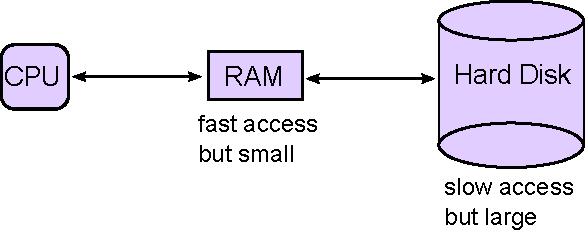
\includegraphics[scale=0.7]{./figures/twoLevelMemory_CPU_RAM_HDD.pdf}
%\caption{Example of a two-level memory hierarchy system}
\end{figure}

The data on the hard disk is divided into blocks called \emph{pages}. When the CPU needs 
to access data the corresponding pages have to be loaded from the hard disk to the RAM such 
that the CPU has fast access to the data. This requires no further action as long as 
the RAM has still some space available. However, if the RAM is full, i.e. there is no room
for new pages from the hard disk, we have to create space for the new page by evicting a page 
from the RAM.

% graphics 
\begin{figure}[h]
\centering
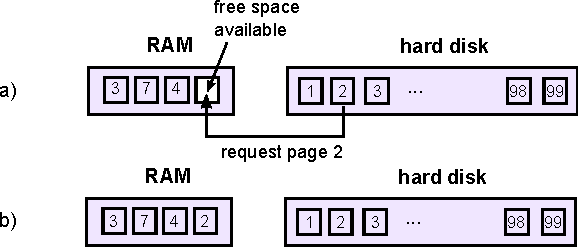
\includegraphics[scale=1.0]{./figures/RAM_hdd_page_part1.pdf}
\caption{a) The RAM has space for 4 pages, and the hard disk consists of 99 pages. Page~2
is requested and loaded from the hard disk to the RAM. b) Page~2 is now in RAM where it can be
accessed by the CPU.}
\end{figure}

% graphics 
\begin{figure}[ht]
\centering
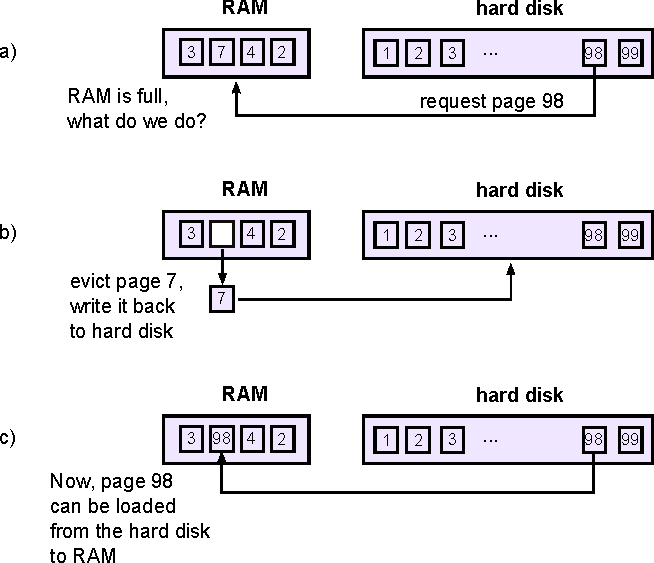
\includegraphics[scale=1.0]{./figures/RAM_hdd_page_part2.pdf}
\caption{a) We request page~98 and try to load it from the hard disk to RAM.
However, the RAM is full. b) We pick an arbitrary page and evict it, e.g. page~7.
c) Now, page~98 can be loaded from the hard disk to RAM.}
\end{figure}

The question is, which page shall we evict? Does it even matter? Indeed, it does. 
Consider these two cases: 
\begin{itemize}
\item Case~1: Suppose we have just evicted page~7 such that it is on 
the hard disk, and our next request is page~7. Then we have to access the hard disk  
to load page~7 to the RAM again.  
\item Case~2: Instead of page~7 we evict page~4. If we request page~7 now,
nothing is to be done. We do not need to load page~7 from the hard disk to RAM since 
page~7 is still in RAM.
\end{itemize}

In case~2 we made a better decision since no access to the hard disk was necessary, 
and recall that accessing the hard disk is slow. 
In general the fast memory is called \emph{cache} and the slow one simply \emph{memory}.
Thus, from now on we will refer to the RAM as cache and the hard disk as memory. 
When we request a page $p$ there are two possibilities: 
\begin{enumerate}
	\item $p$ is in cache and nothing is to be done.
	\item $p$ is not in cache which we will refer to as \emph{cache miss}.
	      If the cache is full, a page has to be evicted such that $p$ can be loaded 
	      from memory to cache (page replacement). 
\end{enumerate}

This is referred to as \emph{paging}~\cite{albers99_brics}. Thus, paging can be understood as memory management where
we have to decide which pages to keep in cache. The goal is to minimize the number of cache misses. 
In the next section we will describe some paging algorithms.


% 1.2 Paging Algorithms
\subsection{Paging algorithms}
We have mentioned that we are trying to minimize the number of cache misses, and that this number
depends on which page we evict. We will describe some paging algorithms that use different page 
replacement policies. An excellent demonstration of the different paging algorithms can be found 
in~\cite{johncctang}. In the following, $k$ is the cache size, i.e. the number of pages that fit in the 
cache, $M$ is the page-set, i.e. the set of all pages, and $\sigma$ is the request sequence.

%1.2.1 Longest Forward Distance (LFD)
\subsubsection{Longest Forward Distance (LFD)}
\label{sec:lfd} 
Suppose we have a cache-size of $k=3$, and the page-set is $M=\{1,2,3,4,5,6\}$.
We request the pages $\sigma=(1,5,3,5,2,6,1,4,3,6,2,5,4,3)$. The algorithm \emph{Longest Forward Distance
(LFD)} evicts the page whose next request lies furthest in the future. Let us have a look at the cache content
in figure~\ref{fig:LFD_example}.

% figure: LFD example
\begin{figure}[h]
	\centering
	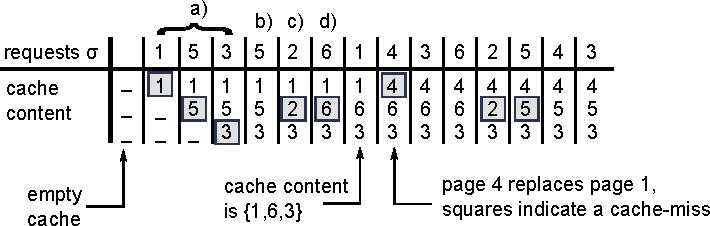
\includegraphics{./figures/LFD_example.pdf}
	\caption{Example for the algorithm LFD processing a request sequence $\sigma$. 
	         The cache size is $k=3$. Numbers enclosed in a square indicate a cache miss.
	         In total there are 8 cache misses.}
	\label{fig:LFD_example}
\end{figure}

\noindent a) In the beginning the cache is empty and is filled by the first three requests 1,5 and 3.
These pages were not in the cache and result in three cache misses.\\
b) The next request is 5, and since 5 is already in the cache nothing is to do. \\
c) Page~2 is requested and is not in cache (cache miss). Since the cache is full we will 
have to evict a page, but which one? According to the LFD policy we evict the page 
whose next request lies furthest in the future, and that is page 5 (see figure~\ref{fig:LFD_example_c}). We evict page~5 and replace it by page~2.

% figure: LFD example, request c)
\begin{figure}[h]
	\centering
	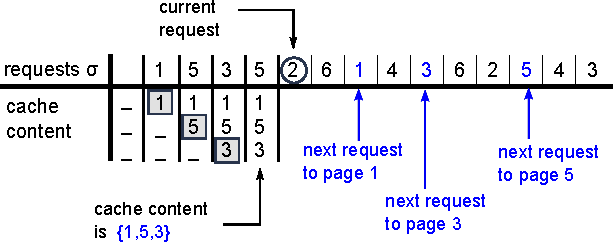
\includegraphics{./figures/LFD_example_c.pdf}
	\caption{The cache content is \{1,5,3\}. Out of these three pages
	         the next request for page 5 lies furthest in the future. Hence, LFD evicts page 5.}
	\label{fig:LFD_example_c}
\end{figure}

\noindent d) Page~6 is requested and is not in cache (cache miss). Again we evict the page 
whose next request lies furthest in the future, and that is page~2 (see figure~\ref{fig:LFD_example_d}). 

% figure: LFD example, request d)
\begin{figure}[h]
	\centering
	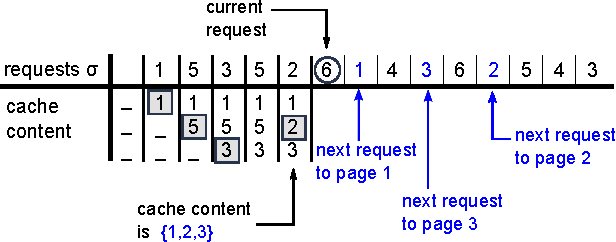
\includegraphics{./figures/LFD_example_d.pdf}
	\caption{The cache content is \{1,2,3\}. Out of these three pages
	         the next request for page 2 lies furthest in the future. Hence, LFD evicts page 2.}
	\label{fig:LFD_example_d}
\end{figure}

In figure~\ref{fig:LFD_example} we can see how LFD processes the whole request sequence $\sigma$. 
There are in total 8 cache misses or 8 page faults. Note that it is common to use the term 
\emph{page fault} instead of cache miss. 

Belady devised LFD and proved in~\cite{belady66_opt} that it is the \emph{optimal} paging algorithm, i.e. there is no other algorithm that yields 
less page faults when processing a request sequence. However, it is not practical since for a current 
request it replaces the page whose next request lies furthest in the future. Knowledge of the future
is usually not available to us.

LFD is called an \emph{offline} paging algorithm which means that at any time the algorithm
can look at the whole request sequence. In contrast, \emph{online} paging algorithms only 
see the current and past requests. Their decision on which page to replace depends only on these
requests.

%1.2.2 Least Recently Used (LRU)
\subsubsection{Least Recently Used (LRU)} 
\emph{Least Recently Used (LRU)} is an online paging algorithm, and as such
decides which page to evict by only looking at the pages that have been requested so far.
It replaces the page that has not been requested for the longest period of time. 
An example will illustrate this policy. Suppose we have a cache size of $k=3$ and the page-set is
$M=\{1,2,3,4,5,6\}$. The request sequence is the same as before, i.e.
 $\sigma = (1,5,3,5,2,6,1,4,3,6,2,5,4,3)$. Let us examine the cache content.

% figure: LRU example
\begin{figure}[h]
	\centering
	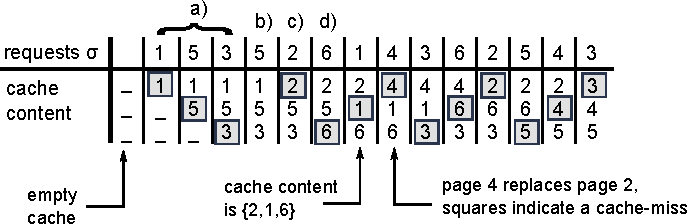
\includegraphics{./figures/LRU_example.pdf}
	\caption{Example for the algorithm LRU processing a request sequence $\sigma$. 
	         The cache size is $k=3$. Numbers enclosed in a square indicate a cache miss.}
	\label{fig:LRU_example}
\end{figure}

\noindent a) The first three requests 1,5 and 3 will just fill the empty cache. These pages have not been
in the cache and evoke three cache misses.\\
b) The next request is 5, and since 5 is already in the cache nothing is to do.\\
c) Page 2 is requested and not in cache (cache miss). Since the cache is full we have to replace a page. 
According to the LRU policy we evict the page that has not been requested for the longest period of time, 
and that is page~1 (see figure~\ref{fig:LRU_example_c}).\\ 
d) Page 6 is requested and not in cache (cache miss). Since the cache is full we have to replace a page. 
According to the LRU policy we evict the page that has not been requested for the longest period of time, 
and that is page~3 (see figure~\ref{fig:LRU_example_d}). 


 % figure: LRU example, request c)
\begin{figure}[ht]
	\centering
	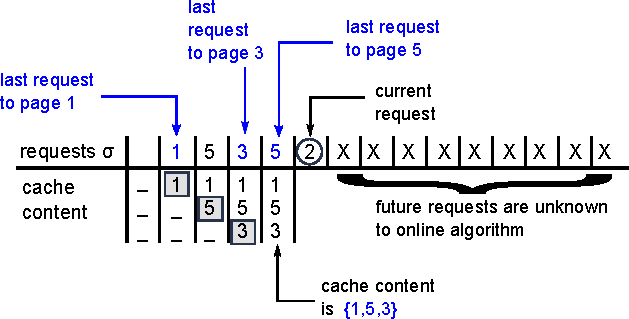
\includegraphics[scale=0.95]{./figures/LRU_example_c.pdf}
	\caption{The cache content is \{1,5,3\}. Out of these three pages
	         1 has not been requested for the longest period of time. Hence, LRU evicts page 1.
	         Notice that the future requests are unknown to LRU.}
	\label{fig:LRU_example_c}
\end{figure}

% figure: LRU example, request d)
\begin{figure}[ht]
	\centering
	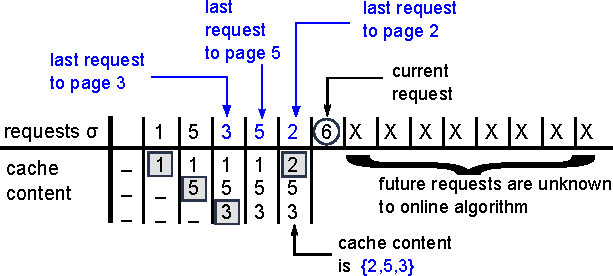
\includegraphics[scale=0.95]{./figures/LRU_example_d.pdf}
	\caption{The cache content is \{2,5,3\}. Out of these three pages
	         3 has not been requested for the longest period of time. Hence, LRU evicts page 3.
	         Notice that the future requests are unknown to LRU.}
	\label{fig:LRU_example_d}
\end{figure}

\noindent In figure~\ref{fig:LRU_example} we can see how LRU processes the whole request sequence.
There are in total 13 page faults.



% COMPETETIVE RATIO
\subsection{Competitive ratio}
There are many more paging algorithms~\cite{albers03_survey}. The question is, how good are they? One popular way to 
gauge the performance of a paging algorithm is to use the \emph{competitive ratio c} which is defined
as follows~\cite{albers99_brics}: 
an algorithm A is \emph{c-competitive} if 
\[ 
\text{A}(\sigma) \leq c \cdot \text{OPT}(\sigma) + b 
\]

\noindent holds for an arbitrary request sequence $\sigma$, where $\text{A}(\sigma$) is the number of cache misses performed by
A, $c$ is the competitive ratio, $\text{OPT}(\sigma)$ is the number of cache misses caused by the optimal paging algorithm OPT and $b$ is some constant. We know from section~\ref{sec:lfd} that LFD is the optimal paging algorithm such that we will refer to LFD as OPT.

Intuitively, the competitive ratio compares the performance of A and OPT. For instance, it is known that LRU 
is $k$-competitive~\cite{sleator85}, where $k$ is the cache size:

\[ \text{LRU}(\sigma) \leq k \cdot \text{OPT}(\sigma) + b \]

\noindent For $k=3$ we have 

\[ \text{LRU}(\sigma) \leq 3 \cdot \text{OPT}(\sigma) + b \]

\noindent which guarantees that in the worst case LRU can only have up to three times as many page faults
as OPT (plus some constant $b$). However, this worst-case guarantee has the drawback of not being 
meaningful in practice. For example, LRU and the algorithm FIFO are both known to be $k$-competitive~\cite{sleator85}, however
LRU performs better in practice than FIFO~\cite{chrobak99}. 

A more experimental approach is to consider a real-world trace, i.e. a long sequence $\sigma$ of page 
requests that has been obtained by tracing memory accesses. For this trace we count the 
number of cache misses by A and OPT respectively and calculate $A(\sigma)/OPT(\sigma)$ which serves
as an empirical competitive ratio~\cite{moruz_soda12}. We typically determine the ratio for different values of $k$ and
plot $A(\sigma)/OPT(\sigma)$ against $k$, see figure~\ref{fig:empirical_ratio}. In order to determine the ratio we obviously need the algorithm OPT for which we will describe an efficient implementation in the next sections. 

% figure: empirical_ratio
\begin{figure}[ht]
	\centering
	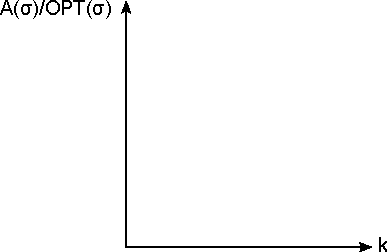
\includegraphics[scale=1.0]{./figures/empirical_ratio.pdf}
	\caption{In experiments the empirical ratio $A(\sigma)/OPT(\sigma)$ is plotted against different cache sizes $k$.}
	\label{fig:empirical_ratio}
\end{figure}


% OPTIMAL OFFLINE PAGING ALGORITHM
\section{Optimal offline paging algorithm}
\subsection{Layer partition}
\label{sec:LayerPartition}
We have mentioned that the Longest Forward Distance algorithm (LFD) yields the minimum number of cache misses
when processing a request sequence. As such we refer to it as the optimal offline paging algorithm OPT meaning
that no other algorithm performs better. It works by evicting the page in cache whose next request lies furthest in the future. 
Obviously, knowledge about the cache content is required. However, Koutsoupias 
and Papadimitriou have found something remarkable in~\cite{koutsoupias00}: when requesting a page it is possible to determine whether 
OPT will perform a cache miss without knowing the precise cache content! Instead a \emph{layer partition} is used. 
Later, a \emph{compressed} version of the layer partition was introduced by Moruz and Negoescu 
in~\cite{sea12_paper} which we will describe here. 

The compressed layer partition $(\cl_0 | \cl_1 | ... | \cl_k)$ consists of $k+1$ layers (disjoint sets) $\cl_0, \cl_1, ..., \cl_k$, where $k$ is the
number of pages that fit in the cache. Each page is in exactly one layer. Example: For $k=3$ we have 
$k+1=4$ layers, and the partition may be given by $(\cl_0 | \cl_1| \cl_2| \cl_3)=(1,3|\emptyset|4,2,5|6).$   

Let $p_1, p_2, ..., p_k$ be the first $k$ pairwise distinct pages in the request sequence $\sigma$, 
and $M$ be the set of all pages. The initial partition is then defined as 

\begin{align*}
& \cl_0 = M \backslash \{ p_1, ..., p_k \} \\
& \cl_1, ..., \cl_{k-1}  \text{ are empty sets} \\
& \cl_k = \{p_1, ..., p_k\} 
\end{align*}

\noindent \textbf{Example 0}: Let $M=\{1,2,3,4,5,6\}$, $k=3$ and $\sigma=(2,5,5,2,1,3,4,6,2,6,4)$. 
The first $k=3$ pairwise distinct requested pages in $\sigma$ are $\{2,5,1\}$, such that the initial 
partition is given by $(\cl_0 | \cl_1| \cl_2| \cl_3)=(3,4,6|\emptyset|\emptyset|2,5,1).$

Upon a request to page $p$ the layer partition is modified according to the following \emph{update rules}, 
where $\cl'_{i}$ is the updated layer and $\cl_{i}$ the old layer:

\begin{center}
\fbox{
\begin{tabular}[ht]{lll}
  \textbf{Case 1:} if $p \in \cl_0$, then        & \hspace{1cm} & \textbf{Case 3:} if $p \in \cl_i, 0<i<k$, then \\
 \quad $\cl'_{0} = \cl_0 \backslash \{p\}$ & \hspace{1cm}& \quad$\cl'_{i-1} = \cl_{i-1} \cup \cl_i \backslash \{p \}$ \\
 \quad $\cl'_{k-1} = \cl_{k-1} \cup \cl_k $   & \hspace{1cm}& \quad$\cl'_k = \cl_k \cup \{ p \}$ \\
 \quad $\cl'_k = \{ p \}$                     & \hspace{1cm}& \quad$\cl'_j = \cl_{j+1}$ for $j=i, i+1, ..., k-2$ \\
 \quad and $\cl'_j=\cl_j$ for $j \ne 0,k-1,k$                     & \hspace{1cm}  & \quad $\cl'_{k-1} = \emptyset$ \\
  \textbf{Case 2:} if $p \in \cl_k$, then         & \hspace{1cm}  &  \quad and $\cl'_j = \cl_j$ for $j=0,...,i-2$  \\
  \quad do nothing                              & \hspace{1cm}  &                                           
\end{tabular}
}
\end{center}

\noindent A more visual representation of the updated layer partition $\cl^p$ is the following:

\[
\boxed{
\cl^p = \begin{cases}
 (\cl_0\backslash\{p\}|\cl_1|\dots|\cl_{k-2}|\cl_{k-1}\cup \cl_k| \{p\} ),
 & \textrm{if } p\in \cl_0 \\ 

 (\cl_0| \cl_1|\dots|\cl_{k-1}| \cl_k  ),
 & \textrm{if } p\in \cl_k \\ 
 
  (\cl_0|\dots|\cl_{i-2}|\cl_{i-1}\cup \cl_{i}\backslash \{p\}| \cl_{i+1}|\dots|\cl_{k-1}| \emptyset|\cl_k\cup \{p\} ),
 & \textrm{if } p\in \cl_i, \\
 &                   0<i<k

\end{cases}
}
\]

\begin{itemize}
	\item \textbf{Case~1}: If $p \in \cl_0$, then $\cl_k$ is merged into $\cl_{k-1}$. Afterwards $p$ is removed
	from $\cl_0$, and the new layer $\cl'_{k}$ contains only $p$.

	\item \textbf{Case~2}: If $p \in \cl_k$, then nothing is to do.
	
	\item \textbf{Case~3}: If $p \in \cl_i$ with $0<i<k$, i.e. $p$ is neither in $\cl_0$ nor in $\cl_k$, 
	then $p$ is removed from $\cl_i$ and inserted in $\cl_k$,
	and $\cl_i \backslash \{p\}$ is merged into $\cl_{i-1}$. Moreover, the content of the layers 
	$\cl_j$ with $j=i+1,i+2,\dots,k-1$ all move one position to the left. As a consequence the new layer $\cl'_{k-1}$ 
	becomes empty.
	
\end{itemize}


\noindent The following examples illustrate the update rules.\\
\\
\textbf{Example 1:}
We consider case~1 with $p\in\cl_0$. The layer partition may be given by

\begin{center}
	\begin{tabular}[ht]{|c|c|c|c|c|}
	  \hline
		$\cl_0$ & $\cl_1$ & $\cl_2$ & $\cl_3$ & $\cl_4$ = $\cl_k$ \\
		\hline		
		9,10 & 7,8 & 5,6 & 3,4 & 1,2 \\
		\hline
	\end{tabular}
\end{center}
 
For the layer partition above we request page $p=9$. Since $p \in \cl_0$, we (1.i) merge $\cl_k$ into
$\cl_{k-1}$:

\begin{center}
	(1.i)
	\begin{tabular}[ht]{|c|c|c|c|c|}
	  \hline
		$\cl_0$ & $\cl_1$ & $\cl_2$ & $\cl_3$ & $\cl_4$ = $\cl_k$ \\
		\hline		
		9,10 & 7,8 & 5,6 & 1,2,3,4 & $\emptyset$ \\
		\hline
	\end{tabular}
\end{center}

(1.ii) We then remove $p$ from $\cl_0$ and finally insert it into the last layer:

\begin{center}
	(1.ii)
	\begin{tabular}[ht]{|c|c|c|c|c|}
	  \hline
		$\cl_0$ & $\cl_1$ & $\cl_2$ & $\cl_3$ & $\cl_4$ = $\cl_k$ \\
		\hline		
		10 & 7,8 & 5,6 & 1,2,3,4 & 9 \\
		\hline

	\end{tabular}
\end{center}

\noindent In case 1 not much happens. Intuitively, page $p$ moves to $\cl_{k}$ and pushes the content of $\cl_k$ one position to the left, to $\cl_{k-1}$.\\

\noindent \textbf{Example 2:}
We consider case~2 with $p \in \cl_k$. The layer partition is given by
\begin{center}
	\begin{tabular}[ht]{|c|c|c|c|c|}
	  \hline
		$\cl_0$ & $\cl_1$ & $\cl_2$ & $\cl_3$ & $\cl_4$ = $\cl_k$ \\
		\hline		
		9,10 & 7,8 & 5,6 & 3,4 & 1,2 \\
		\hline
	\end{tabular}
\end{center}
We request page 2 and then page 1. This requires no further action since both pages are in $\cl_k$.\\
\\
\noindent \textbf{Example 3:} We consider case~3 with $p \in \cl_i, 0<i<k$. The layer
partition is given by
\begin{center}
	\begin{tabular}[ht]{|c|c|c|c|c|}
	  \hline
		$\cl_0$ & $\cl_1$ & $\cl_2$ & $\cl_3$ & $\cl_4$ = $\cl_k$ \\
		\hline		
		9,10 & 7,8 & 5,6 & 3,4 & 1,2 \\
		\hline
	\end{tabular}
\end{center}

We request page $p=7$. Since $p \in \cl_i$ with $0<i<k$, i.e. $p$ is neither from $\cl_0$ nor $\cl_k$, 
we do the following: 

\noindent (3.i) $p=7$ is removed from $\cl_i=\cl_1$ and inserted in $\cl_k$:
\begin{center}
	(3.i)
	\begin{tabular}[ht]{|c|c|c|c|c|}
	  \hline
		$\cl_0$ & $\cl_1$ & $\cl_2$ & $\cl_3$ & $\cl_4$ = $\cl_k$ \\
		\hline		
		9,10 & 8 & 5,6 & 3,4 & 1,2,7 \\
		\hline
	\end{tabular}
\end{center}

\noindent (3.ii) $\cl_i \backslash \{p\}=\{8\}$ is merged into $\cl_{i-1}$:
\begin{center}
	(3.ii)
	\begin{tabular}[ht]{|c|c|c|c|c|}
	  \hline
		$\cl_0$ & $\cl_1$ & $\cl_2$ & $\cl_3$ & $\cl_4$ = $\cl_k$ \\
		\hline		
		8,9,10 & $\emptyset$ & 5,6 & 3,4 & 1,2,7 \\
		\hline
	\end{tabular}
\end{center}

\noindent (3.iii) The contents of layers $\cl_2$ and $\cl_3$ move one position to the left.
The new layer $\cl_{k-1}=\cl_3$ is empty now:
\begin{center}
	(3.iii)
	\begin{tabular}[ht]{|c|c|c|c|c|}
	  \hline
		$\cl_0$ & $\cl_1$ & $\cl_2$ & $\cl_3$ & $\cl_4$ = $\cl_k$ \\
		\hline		
		8,9,10 &  5,6 & 3,4 & $\emptyset$ & 1,2,7 \\
		\hline
	\end{tabular}
\end{center}

\noindent The formal description of case~3 may look complicated but is 
actually easy to understand. Intuitively, if we request a page $p\in \cl_i$ with $0<i<k$, 
then all the layers from $\cl_i$ to $\cl_{k-1}$ jump one position to the left, and as a 
consequence $\cl_{k-1}$ becomes empty. Then page $p$ is moved to $\cl_k$. \\
\\
\noindent \textbf{Example 4}: We also want to consider how the layer partition processes a whole 
request sequence $\sigma$ from beginning to end. Let $M=\{1,2,3,4,5,6\}$ be the page-set, $k=3$ 
the cache size and $\sigma=(4,2,4,5,6,4,1,2,1,6,2,4)$ the request sequence. 

The first $k=3$ pairwise distinct requested pages are $\{4,2,5\}$,  
from which we can deduce the initial partition 
$(\cl_0 | \cl_1| \cl_2| \cl_3)=(1,3,6|\emptyset|\emptyset|4,2,5)$, see also example 0.  
Table~\ref{tab:example4} shows the requests after these first 3 distinct pages. \\

\begin{table}
\begin{center}
	\begin{tabular}[ht]{|c||c|c|c|c||c|}
	  \hline
		request &  $\cl_0$ & $\cl_1$ & $\cl_2$ & $\cl_3 = \cl_k$ & OPT \\
		\hline	
		4,2,5		& 1,3,6 	& $\emptyset$ 	&	 $\emptyset$	 &	4,2,5 &  3 cache misses \\
		\hline
	  $6 \in \cl_0$	& 1,3			& $\emptyset$		&  4,2,5				 &  6			&  1 cache miss\\
		\hline
		$4 \in \cl_2$ & 1,3			& 2,5           &  $\emptyset$   &  6,4   & \\
		\hline
		$1 \in \cl_0$ & 3       & 2,5           &  6,4           &  1     & 1 cache miss\\
		\hline
		$2 \in \cl_1$ & 3,5     & 6,4           & $\emptyset$    &  1,2    & \\
		\hline
		$1 \in \cl_3$ & 3,5     & 6,4           & $\emptyset$    &  1,2  & \\
		\hline
		$6 \in \cl_1$ & 3,5,4   & $\emptyset$   & $\emptyset$    & 1,2,6 & \\
		\hline
		$2 \in \cl_3$ & 3,5,4   & $\emptyset$   & $\emptyset$    & 1,2,6 & \\
		\hline
		$4 \in \cl_0$ & 3,5     & $\emptyset$   & 1,2,6          & 4     & 1 cache miss \\ 
		\hline
		
	\end{tabular}
	\caption{Illustration of example 4. The layer partition processes a request sequence $\sigma$.
	The second line shows the initial partition after the first $k=3$ pairwise distinct pages in $\sigma$.
	The last column describes OPT's behaviour according to property (Pr1). There are in total 6 cache misses.}
	\label{tab:example4}
\end{center}
\end{table}

\noindent Now, the layer partition has an interesting property~\cite{moruz_soda12}: \\
\\
\textbf{Property (Pr1):} After the first $k$ pairwise distinct requested pages 
OPT will perform a cache miss upon a request to page $p$, if and only if $p \in \cl_0$ in the layer partition.\\
%\textbf{Property (P1):} Upon a request to page $p$ the optimal paging algorithm \\
%OPT will perform a cache miss, if and only if $p \in \cl_0$ in the layer partition. \\
\\
Let us examine what this means for the request sequence in example~4. In table~\ref{tab:example4} 
we see that there are 3 requests with $p \in \cl_0$ (pages 6,1,4). OPT will perform a cache miss for these
requests according to (Pr1) such that we have 3 page faults. 

Moreover, we know that OPT's cache is empty in the beginning, so the first $k=3$ pairwise distinct requested pages
could not have been in the cache and lead to 3 additional cache misses. In total OPT should 
have performed 3+3=6 page faults. We should check this using the LFD policy from section~\ref{sec:lfd}.

% figure: LFD for comparison with layer partition
\begin{figure}[h]
	\centering
	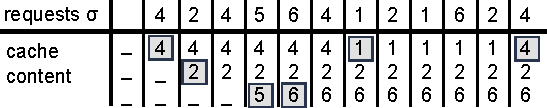
\includegraphics{./figures/LFD_compare_layerPartition2.pdf}
	\caption{The algorithm LFD processing the request sequence $\sigma$ from example~4.
					 Squares indicate a cache miss. There are in total 6 page faults.}
	\label{fig:LFD_compare_layerPartition2}
\end{figure}


\noindent As you can see in figure~\ref{fig:LFD_compare_layerPartition2} there are indeed 6 page faults. Compare figure~\ref{fig:LFD_compare_layerPartition2} with table~\ref{tab:example4}
and notice how OPT will perform a cache miss, if and only if the requested page is from $\cl_0$ in the layer partition
(after the first $k$ pairwise distinct requested pages in the beginning). 

This is quite a remarkable result since it allows us to determine whether OPT will perform a page fault without 
using the LFD policy! Instead, all we have to do is use the layer partition. Notice that when we use the LFD policy
we form OPT's cache content. In contrast, when we use the layer partition we do not know the precise content of OPT's cache (see appendix). 
The question is, how do we implement the layer partition efficiently? We will answer this in the next sections.  
 

\subsection{Union-Find data structure}
We have seen that the update rules for the layer partition include the union of disjoint sets, namely the layers. 
Galler and Fischer~\cite{galler64} developed an efficient \emph{union-find} data structure to maintain elements that are partitioned in disjoint sets. Each set consists of a tree of elements with a parent pointer, and is 
represented by the root whose parent pointer points to itself.\\
Example: Suppose we have the set $S=\{1,2,...,8\}$ that is partitioned into $P_1=\{1,2\}$, $P_2=\{3,4,5,6,7\}$, 
$P_3=\{8\}$. This partition may be represented by the trees in figure~\ref{fig:gallerFischer_example}. 

% figure: example for galler fischer tree data structure
\begin{figure}[h]
	\centering
	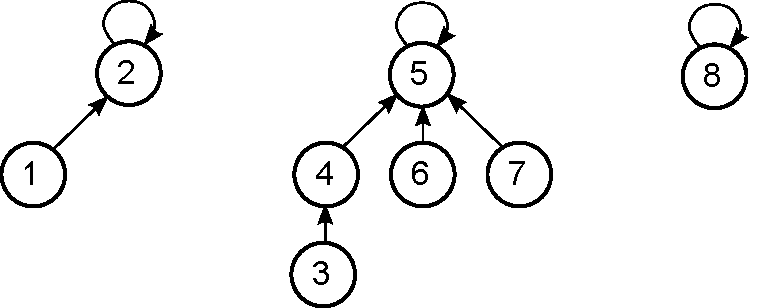
\includegraphics[scale=0.5]{./figures/gallerFischer_example.pdf}
	\caption{Example for the Galler-Fischer tree data structure. The trees represent the sets
					$P_1=\{1,2\}$, $P_2=\{3,4,5,6,7\}$ and $P_3=\{8\}$.}
	\label{fig:gallerFischer_example}
\end{figure}

\noindent A root is identified by checking if the parent pointer points to itself. This is the 
case for elements 2, 5 and 8. The root denotes the set, e.g. 5 represents $P_2$. This allows us 
to determine whether two elements are in the same set simply by comparing their roots. For instance, 
3 and 7 belong to the same set since their root is 5. 

The data structure supports three operations: \emph{union}, \emph{find} and \emph{makeset}. 
The \emph{find} operation determines in which set an element is by following the parent pointers
till the root. The \emph{union} operation on two sets works by linking the root of one tree
to the root of the other tree, see figure~\ref{fig:gallerFischer_example1}. A \emph{makeset} operation 
creates a node with a parent pointer pointing to itself.

% figure: example for galler fischer tree data structure union operation
\begin{figure}[ht]
	\centering
	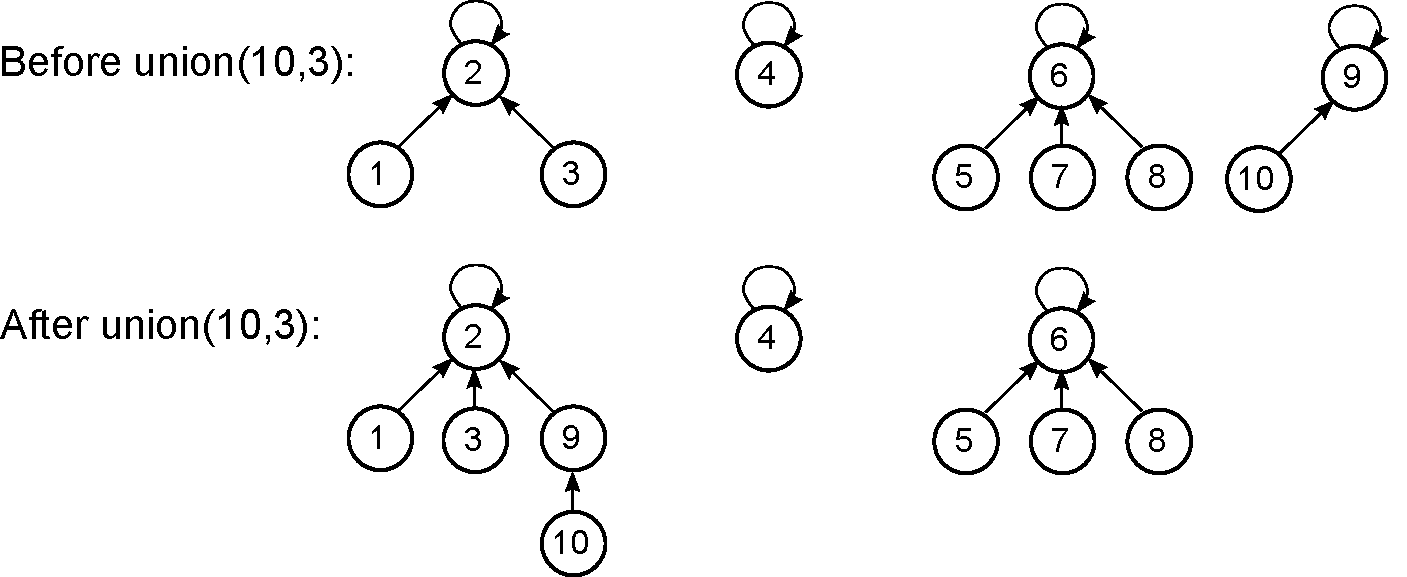
\includegraphics[scale=0.47]{./figures/gallerFischer_example1.pdf}
	\caption{Example for a union operation in the Galler-Fischer tree data structure. 
	        Union(10,3) is performed by first finding the root of 10 and 3 respectively via find(10) and
	        find(3). The root of 10 is then linked to the root of 3.}
	\label{fig:gallerFischer_example1}
\end{figure}

\noindent \emph{Union by rank}. Under certain circumstances a find operation can be expensive, e.g. if we have elements 
$1,2, ...,n$ and apply the consecutive operations union(1,2), union(2,3), ..., union($n$-1,$n$), then 
a tree of height $n-1$ is generated. A find operation will then require $\theta(n)$ time in the worst case.

A technique known as \emph{union by rank}~\cite{tarjan83} prevents this by considering the \emph{rank} which 
is an upper bound for the height of a tree~\cite{tarjan_leeuwen84, tarjan_golumbic}. The tree with smaller rank is then linked to the tree with greater rank, 
see figure~\ref{fig:gallerFischer_unionByRank}.
This keeps the trees flat and guarantees that a union or find operation will run in $\mathcal{O}(\log(n))$ time. 

% figure: union by rank
\begin{figure}[ht]
	\centering
	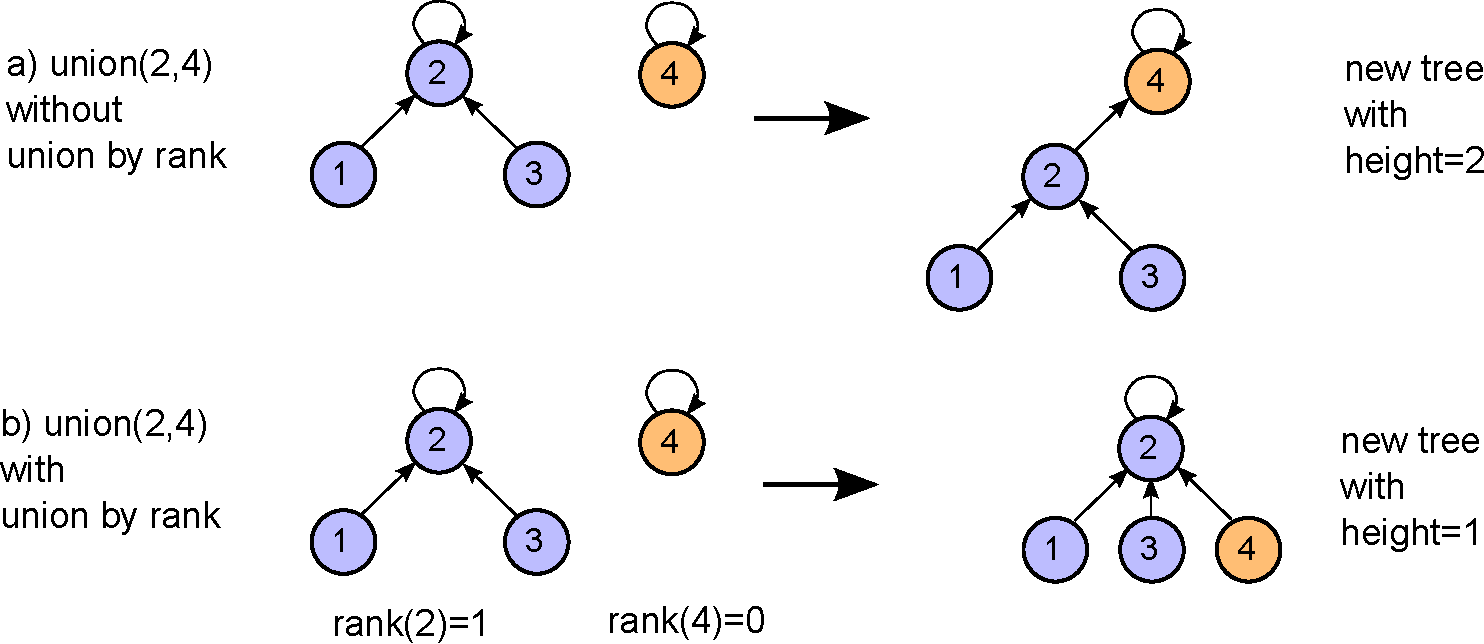
\includegraphics[scale=0.5]{./figures/gallerFischer_unionByRank.pdf}
	\caption{Two trees are unified via union(2,4). In a) the union is performed without union by rank which
	        generates a tree of height 2. In contrast, b) is performed with union by rank, i.e. the tree with smaller
	        rank is linked to the tree with greater rank. This yields a tree of height 1.}
	\label{fig:gallerFischer_unionByRank}
\end{figure}

\noindent \emph{Path compression.} The find operation involves following the parent pointers until we reach the
root $r$. However, we can improve the runtime if we traverse the path to $r$ for a second time and link 
each node we pass directly to $r$, see figure~\ref{fig:gallerFischer_pathCompression}. This \emph{path compression} will make subsequent find operations 
for these attached nodes and their children faster. 

% figure: path compression
\begin{figure}[ht]
	\centering
	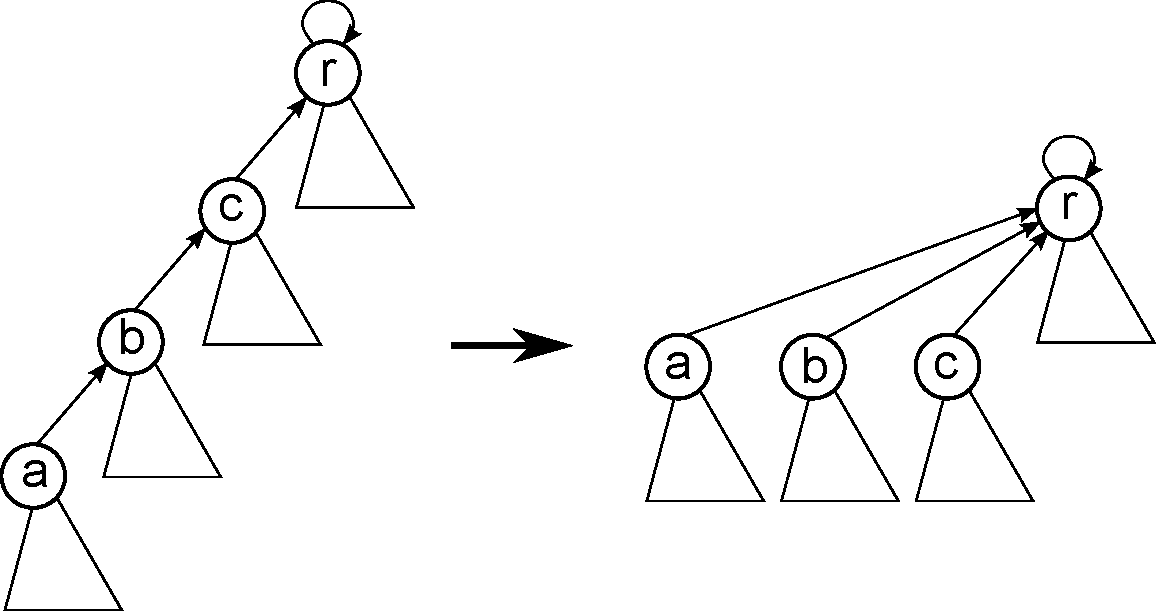
\includegraphics[scale=0.4]{./figures/gallerFischer_pathCompression.pdf}
	\caption{find(a) follows the parent pointers until node $r$ passing the nodes $b$ and $c$.
	         In a second traversal $a$, $b$ and $c$ are directly linked to $r$. Subsequent find 
	         operations for $a$, $b$, $c$ and their children (nodes in subtrees) run faster.}
	\label{fig:gallerFischer_pathCompression}
\end{figure}

Using union by rank together with path compression Tarjan showed the following 
in~\cite{tarjan_golumbic, tarjan83, tarjan75}: 

\textbf{Tarjan's result}: Let $n$ be the number of elements, each one in a 
different set such that we have $n$ singleton sets. Performing $\mu$ union- or find operations 
on these sets (with $\mu \geq n$) requires $\mathcal{O}(\mu \cdot \alpha(n))$ time, where $\alpha(n)$ is a very
slowly growing function known as inverse Ackermann function~\cite{inverse_ackermannFunction}. 

Note that the \emph{amortized runtime} per operation is $\mathcal{O}(\alpha(n))$, which is effectively 
constant since $\alpha(n)$ is smaller than 5 for all practical values of $n$, see~\cite{jeffe}. 
 To emphasize the meaning of this
let us review the runtime improvements for the union-find data structure by Galler and Fischer for $n$ elements
and $\mu \geq n$ operations:

\begin{itemize}
	\item No union by rank and no path compression: \\
		runtime = $\mu \cdot \mathcal{O}(n)$, since the worst-case requires $\theta(n)$ time
	\item Union by rank, but no path compression: \\
	  runtime = $\mu \cdot \mathcal{O}(\log(n))$
	\item Union by rank with path compression: \\
	  runtime = $\mu \cdot \mathcal{O}(\alpha(n))$, approximately $\mu \cdot \oh(1)$
\end{itemize}

\noindent A nice java-applet that demonstrates this union-find data structure can be found in~\cite{gallerFischer_javaApplet}.
Note that during path compression the rank, which is an upper bound for the height, does not change~\cite{brPreiss_onlineBook}.

% SUBSECTION: Implementing the layer partition--------------------------------------
\subsection{Linked trees implementation of the layer partition (LTrees)}
The update rules for the layer partition include the \emph{union} of disjoint sets and
the \emph{deletion} of an element from a set. It is therefore obvious to adopt the 
union-find tree data structure by Galler and Fischer. However, we have to modify it 
since it does not support the deletion of elements, and deleting an element efficiently is not a trivial task.
Here, we had the idea~\cite{andrei_idea} of using \emph{lazy deletion}, i.e. we do not immediately
delete a node but instead mark it. Marked nodes are then deleted in batches. 

We implement the layer partition as follows: each layer is represented by a tree, and the roots 
of adjacent layers are linked to each other, see figure~\ref{fig:layerPartitionTrees2}.

% figure: layerPartitionTrees2
\begin{figure}[ht]
	\centering
	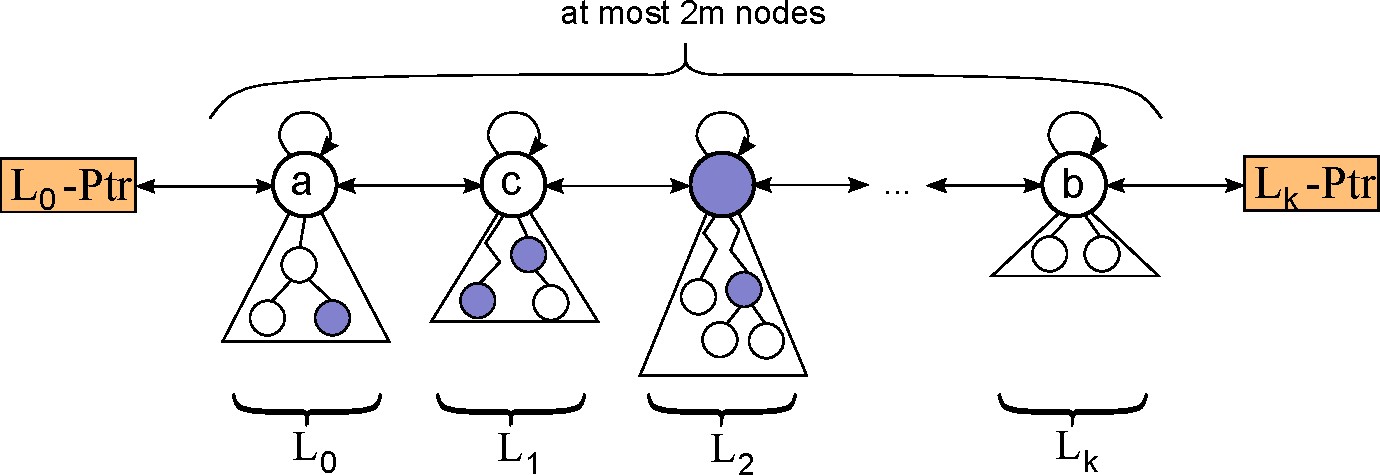
\includegraphics[scale=0.5]{./figures/layerPartitionTrees2.pdf}
	\caption{The data structure for the layer partition $(\cl_0 | \cl_1 | ... | \cl_k)$.
					Each layer is represented by a tree. 
	         $\cl_0$-Ptr and $\cl_k$-Ptr are special 
	         pointers used to decide whether a page is in $\cl_0$ or $\cl_k$. The trees 
	         with root nodes $a$ and $b$ represent layers $\cl_0$ and $\cl_k$ respectively. 
	         Filled nodes are marked as deleted. There are at most $k+1$ trees with $k$ being the cache size. The total number of nodes
	         is restricted to $2m$, where $m$ is the page-set size.}
	\label{fig:layerPartitionTrees2}
\end{figure}

Recall that we need to determine whether a page $p$ is in $\cl_0$, $\cl_k$ or in $\cl_i$ with $0<i<k$
in order to apply the appropriate update rule. This can be done with the help of the pointers 
$\cl_0$-Ptr, $\cl_k$-Ptr and the find($p$) operation which returns the root of $p$: 
\begin{itemize}
 \item If $a$=$\text{find}(p)$, i.e. $a$ is the root of $p$, 
       and $\cl_0$-Ptr points to $a$, then $p$ is in $\cl_0$ (see root node $a$ 
       in figure~\ref{fig:layerPartitionTrees2}).
 
 \item If $b$=$\text{find}(p)$, i.e. $b$ is the root of $p$, and $\cl_k$-Ptr points to $b$, then $p$ is in $\cl_k$ (see
 	root node $b$ in figure~\ref{fig:layerPartitionTrees2}).
 
 \item If $c$=$\text{find}(p)$, i.e. $c$ is the root of $p$, and neither $\cl_0$-Ptr nor $\cl_k$-Ptr point to $c$, then
       $p$ is in $\cl_i$ with $0<i<k$ (see e.g. root node $c$ in figure~\ref{fig:layerPartitionTrees2}). 
\end{itemize}

\noindent Empty layers are not represented by a tree. Instead every root node has a variable \emph{count} that 
stores the number of consecutive empty sets that are adjacent to the left, see 
figure~\ref{fig:LTrees_countVariable}.

% figure: Ltrees_countVariable
\begin{figure}[ht]
	\centering
	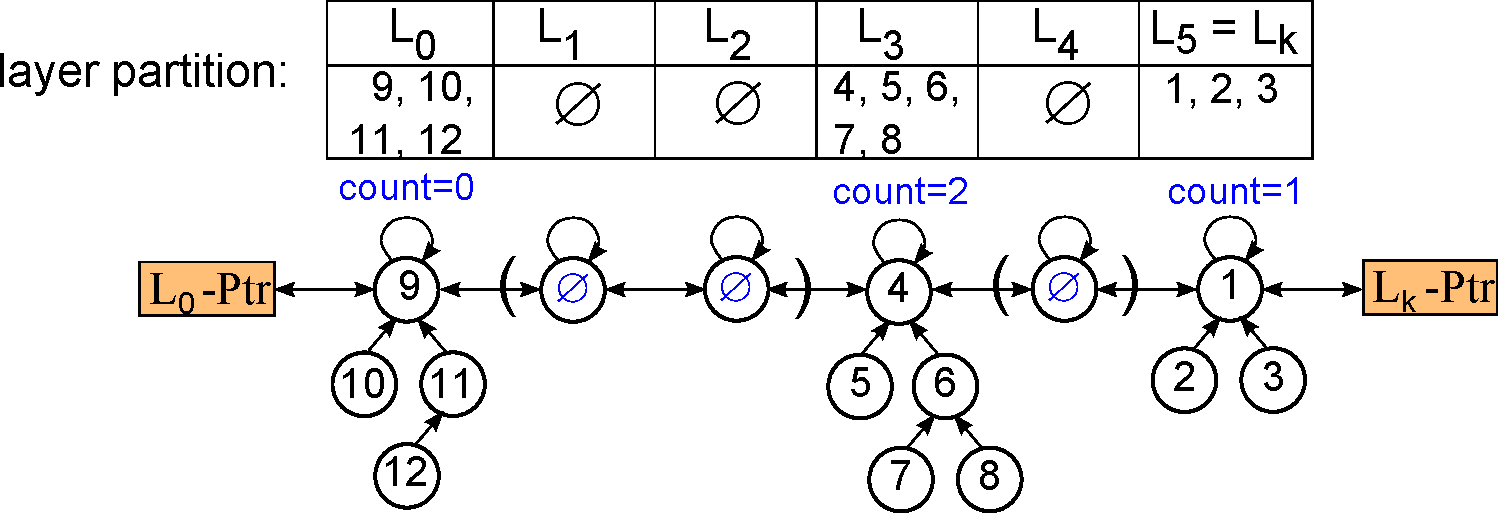
\includegraphics[scale=0.43]{./figures/LTrees_countVariable_small.pdf}
	\caption{The layer partition is represented by the linked trees. The count variable describes 
	         the number of empty sets adjacent to the left. The nodes with empty sets do not exist and 
	         are only drawn for illustration purposes.}
	\label{fig:LTrees_countVariable}
\end{figure}

\noindent The update rules upon request to page $p$ are implemented as follows: 
\begin{itemize}
\item Case (i): If $p \in \cl_0$, then $\cl_k$ is merged into $\cl_{k-1}$. Afterwards, $p$ is removed from
    $\cl_0$ and inserted as new layer $\cl'_k$ such that $\cl'_k=\{p\}$.
    
    This is done by marking the corresponding node for $p$ in the tree of $\cl_0$ as deleted
    and inserting a new node for $p$ as new layer $\cl'_k=\{p\}$. The union of $\cl_k$ and $\cl_{k-1}$
    is performed by linking the root node in $\cl_k$ to the root node in $\cl_{k-1}$,
    (or vice versa link the root node in $\cl_{k-1}$ to $\cl_k$ depending on the ranks) 
    see figure~\ref{fig:LTrees_case1}. If $\cl_{k-1}$ is empty, such that $\cl_{k}$ is merged
    with an empty layer, then the count variable for layer $\cl_k$ is decremented since the number
    of empty sets to the left decreases.  
    
\item Case (ii): If $p \in \cl_k$, then nothing is to do. 
\item Case (iii): If $p \in \cl_i$ with $0<i<k$, then $p$ is removed from $\cl_i$ and added to $\cl_k$.
                 Afterwards $\cl_i \backslash \{p\}$ is merged into $\cl_{i-1}$, and an empty set is inserted as 
		    new layer $\cl'_{k-1}$ such that $\cl'_{k-1}=\emptyset$.
	
		    This is done by marking the corresponding node for $p$ in the tree of $\cl_i$ as deleted 
		    and linking a new node for $p$ to the tree of $\cl_k$. The trees of $\cl_i$ and $\cl_{i-1}$
                 are then merged (alternatively, if $\cl_{i-1}$ is empty, then the count variable for $\cl_i$ is decremented). 
                  Inserting an empty set as $\cl'_{k-1}$ is performed by increasing the count
                 variable of the root node in $\cl_k$, see figure~\ref{fig:LTrees_case3}.  
\end{itemize}

\noindent Note that in (i) and (ii) we can check efficiently whether $p$ is in $\cl_0$ or $\cl_k$ with the help
of the pointers $\cl_0$-Ptr and $\cl_k$-Ptr. In contrast, in (iii) we cannot determine efficiently the index $i$
for a page $p \in \cl_i$~\cite{LTrees_find_index_i}.

% figure: Ltrees_case1
% use htp to force latex to put two figures on same page, see
% http://en.wikibooks.org/wiki/LaTeX/Floats,_Figures_and_Captions
\begin{figure}[htp]   
	\centering
	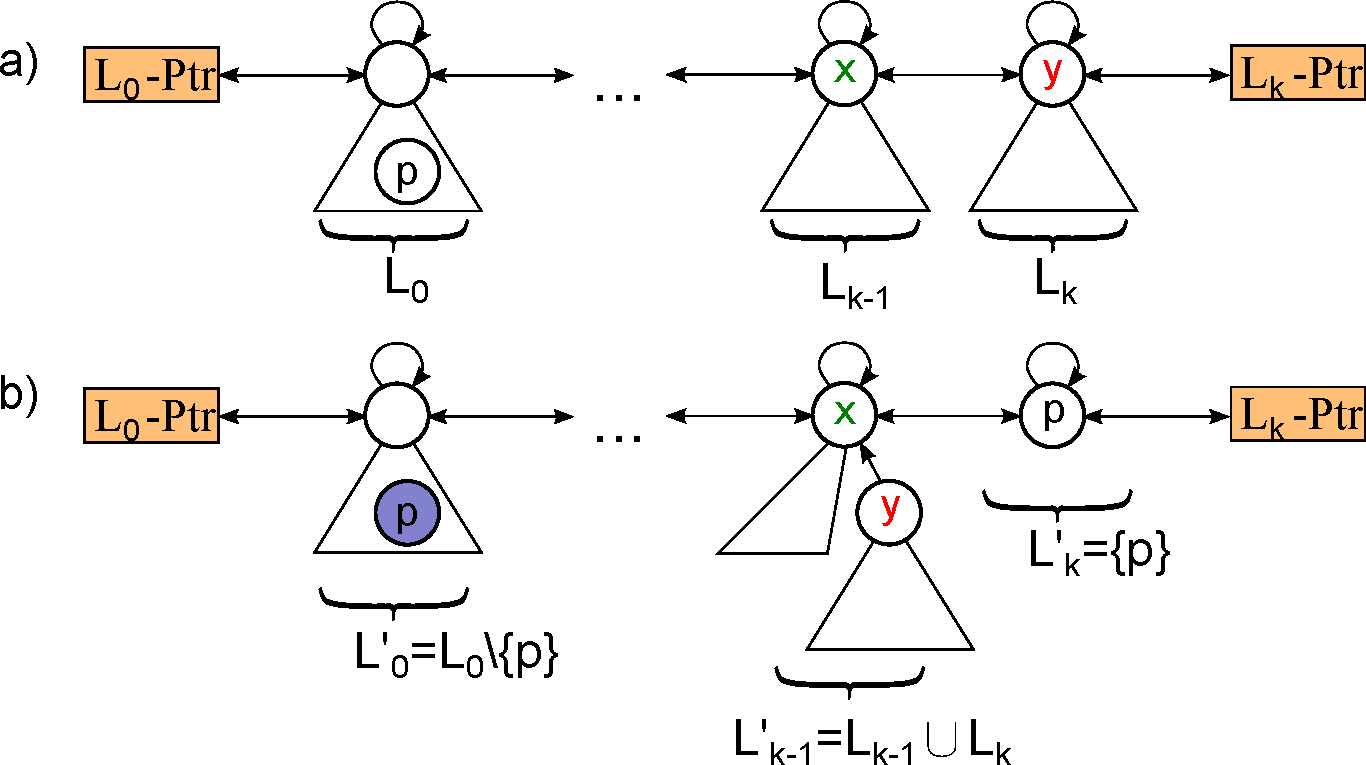
\includegraphics[scale=0.5]{./figures/LTrees_case1.pdf}
	\caption{Implementation of case 1 of the update rules for the layer partition. 
	         a) shows the data structure before and b) after the request to page $p \in \cl_0$.
	         The filled node represents a node that is marked as deleted. Node $y$ is linked to node $x$.
	         (or vice versa $x$ is linked to $y$ depending on the ranks).}
	\label{fig:LTrees_case1}
\end{figure}

% figure: Ltrees_case3
\begin{figure}[htp]
	\centering
	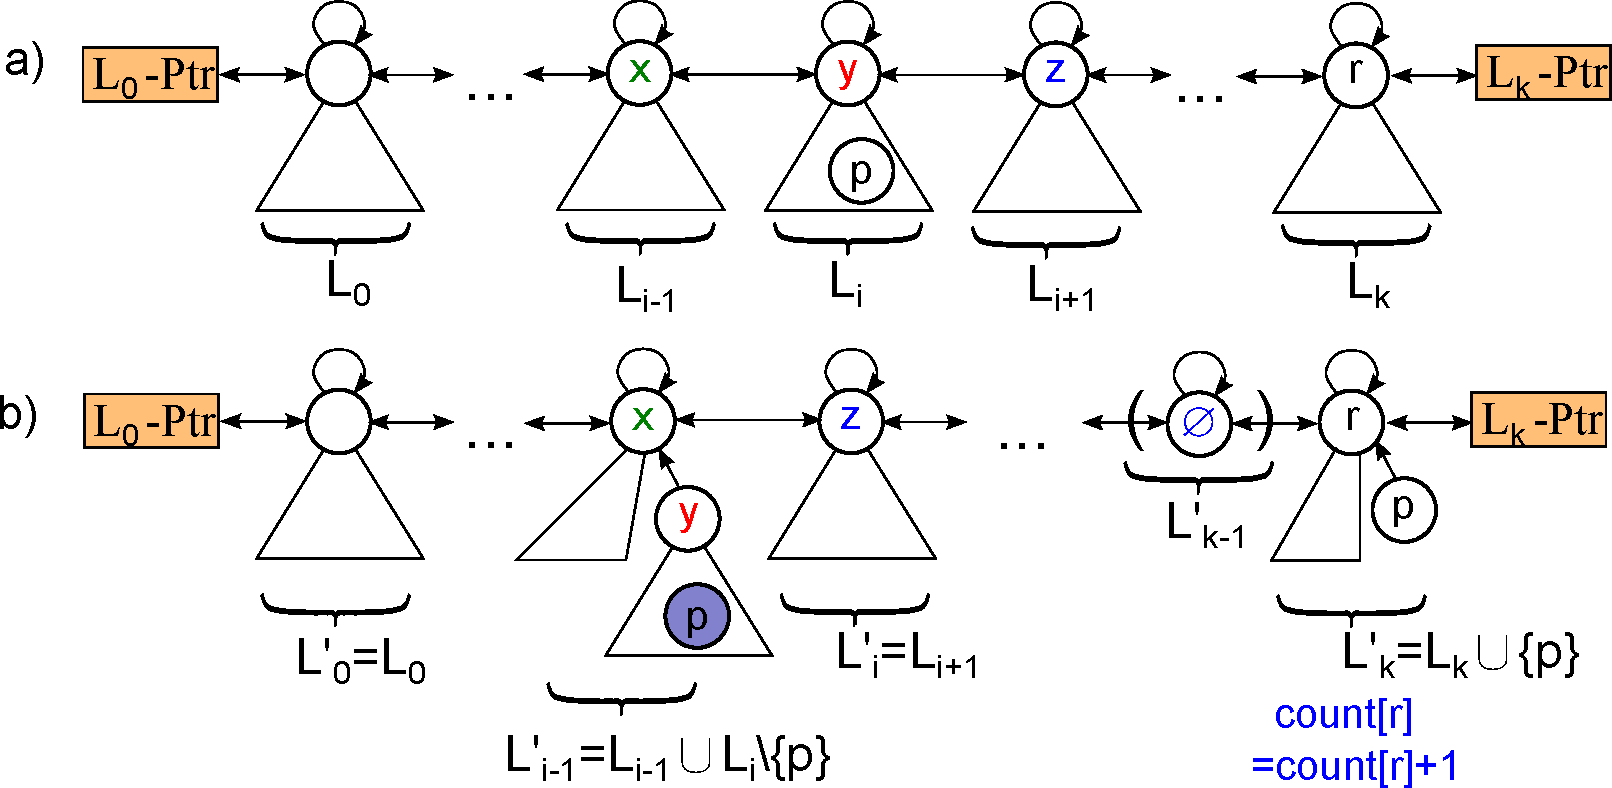
\includegraphics[scale=0.5]{./figures/LTrees_case3.pdf}
	\caption{Implementation of case 3 of the update rules for the layer partition. 
	         a) shows the data structure before and b) after the request to page $p \in \cl_i$
	         with $0<i<k$.
	         The filled node represents a node that is marked as deleted.
	         An empty set is inserted by increasing the count variable of node $r$.
                 Node $y$ is linked to node $x$ 
	         (or vice versa $x$ is linked to $y$ depending on the ranks).} 
	\label{fig:LTrees_case3}
\end{figure}

\subsubsection{Cleanup procedure for LTrees}
\noindent \emph{Lazy deletion.} In the cases $p \in \cl_0$ and $p \in \cl_i$ with $0<i<k$ the number 
of nodes increases by one since we mark the old node for $p$ and insert a new node for $p$. To prevent
an arbitrary growth of the data structure we will restrict the number of nodes to $2m$, where $m$ is the 
is the page-set size. If the total number of nodes reaches the value $2m$, i.e. there are $m$ regular and $m$ marked
nodes, we perform a cleanup procedure. The cleanup procedure removes all marked nodes and consists of the following steps (see figure~\ref{fig:LTrees_cleanup}):\\
\\
\textit{Step 1}: 
Apply a find operation with path compression to all $2m$ nodes. This step creates trees with a height of at most 1.\\
\\
\textit{Step 2}:
Half of the nodes are marked as deleted. We remove them as follows:\\
For all nodes $u$: \\
Case 1: If $u$ is a root, do nothing \\
Case 2: If $u$ is a child: \\
\hspace*{.5cm} if $u$ is marked as deleted, then remove the node \\
\hspace*{.5cm} if $u$ is not marked as deleted: \\
                  \hspace*{1cm} if parent (root) of $u$ is not marked as deleted, then do nothing \\
                  \hspace*{1cm} if parent (root) of $u$ is marked as deleted, then replace the root by $u$ \\
\\
\textit{Step 3}: After step 2 there may still be some marked root nodes without children. 
These will be removed by simply going through all root nodes.\\


% figure: Ltrees_cleanup
\begin{figure}[htp]
	\centering
	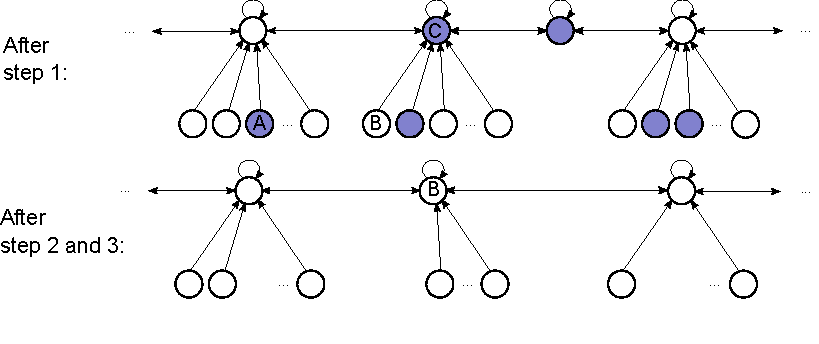
\includegraphics[scale=1.0]{./figures/LTrees_cleanup.pdf}
	\caption{Cleanup procedure: After step 1 all trees have height of at most 1. Filled nodes represent 
	nodes that are marked as deleted. In step 2 and 3 marked nodes are removed. Node A is removed. 
	Node B replaces node C.} 
	\label{fig:LTrees_cleanup}
\end{figure}

\noindent We will refer to this data structure as \emph{LTrees} which stands for \textbf{L}inked \textbf{T}rees.
Recall that LTrees implements the layer partition and can therefore tell us whether OPT will perform a cache miss
upon a page request.

\subsubsection{Runtime analysis for LTrees}
When a page $p$ is requested we pass it to our linked trees data structure which applies the appropriate update
rule and tells us whether OPT will perform a cache miss. The question is, how much time LTrees needs to process
the request. There are two phases, see figure~\ref{fig:LTrees_analysis}.

% figure: Ltrees_cleanup
\begin{figure}[htp]
	\centering
	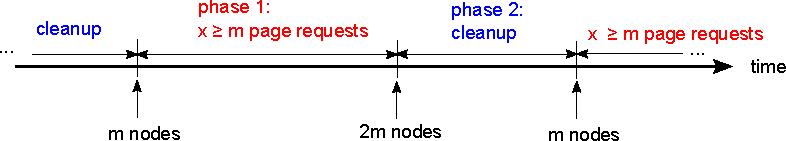
\includegraphics[scale=0.9]{./figures/LTrees_analysis.pdf}
	\caption{There are two phases for LTrees. In phase 1 we start with $m$ nodes and request pages until we 
		have $2m$ nodes. 
                    Then in phase 2 the cleanup procedure takes place removing $m$ marked nodes.} 
	\label{fig:LTrees_analysis}
\end{figure}

\noindent \textbf{Runtime for phase 1:}\\
\noindent - At the beginning of phase~1 we have exactly $m$ regular nodes in LTrees, namely one node for each page, 
where $m$ is the page-set size. \\
\\
- As we request pages, LTrees grows in the cases where $p\in\cl_0$ and $p\in\cl_i$ with $0<i<k$ until 
it consists of $2m$ nodes. Since we start with $m$ nodes we need at least $m$ requests to reach the size 
of $2m$ nodes. \\
\\
- We could need more than $m$ requests because a request does not necessarily add a node to LTrees
(case $p\in\cl_k$). Thus, in phase~1 we perform $x \geq m$ page requests until the data structure consists of $2m$ nodes.\\
\\
- Each request requires at least a find operation (to determine in which layer a requested page $p$ is) and possibly
a union operation (cases $p\in\cl_0$ and $p\in\cl_i$ with $0<i<k$) yielding at most $2x$ union or find operations. 
Since the union and find operation require $\oh(\alpha(2m))$ time according to Tarjan's result, the total runtime $t_1$ for phase~1 is
 
\[
t_1 = 2x \cdot \oh(\alpha(2m))=x \cdot \oh(\alpha(2m)).
\]

\noindent - However, note that Tarjan's result assumes that we start with $m$ singleton sets (situation A). 
Instead at the beginning of phase~1 we have $m$ nodes, and some of them form trees of height~1 (situation B), see again 
figure~\ref{fig:LTrees_cleanup}. Thus not all trees represent singleton sets as opposed to situation A. The question is, are we allowed to use Tarjan's result?

We can use Tarjan's result if we pretend having started at situation A and getting to situation B with the following \emph{transformation}, 
see figure~\ref{fig:LTrees_transformation}.
In situation A we have $m$ singleton sets. We first perform at most $m-1$ union operations to get trees of height~1
($m-1$ is the maximum number of union operations we can perform on $m$ elements until all elements are in the same tree). 
To finally arrive at situation B we link $k+1$ root nodes to each other and 
set the pointers $\cl_0$-Ptr and $\cl_k$-Ptr which requires $k \cdot \oh(1)$ time. The root nodes can be found by applying 
$m$ find operations. In summary, the transformation and the $x$ page requests imply
\begin{align*}
1. \quad &(m-1)  \text{ union operations }  \\
2. \quad & \text{linking roots requiring $k \cdot \oh(1)$ time} \\
3. \quad & m \text{ find operations } \\
4. \quad & 2x \text{ union or find operations }
\end{align*}
\noindent Therefore, we have $[(m-1)+m+2x]$ union or find operations each taking 
$\oh(\alpha(2m))$ time.
% figure: Ltrees_cleanup
\begin{figure}[htp]
	\centering
	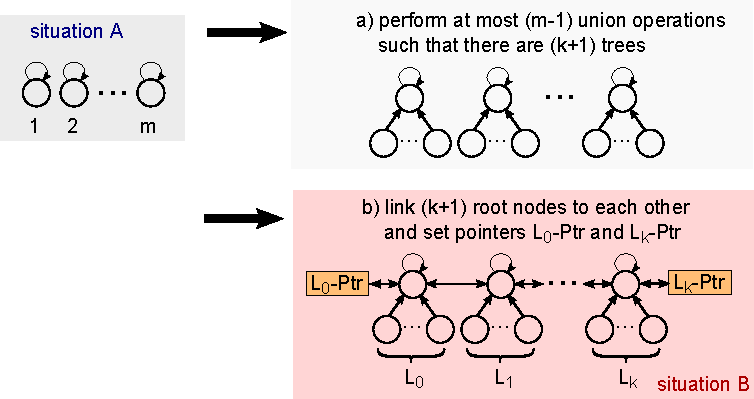
\includegraphics[scale=1.0]{./figures/LTrees_transformation.pdf}
	\caption{The transformation starting from situation A and ending in situation B. Situation B corresponds to LTrees right after a cleanup procedure, 
                     see also figure~\ref{fig:LTrees_cleanup}.} 
	\label{fig:LTrees_transformation}
\end{figure}

Let us see what happens if we include the transformation before phase~1. 
The runtime $t'_1$ including the transformation is calculated as follows
(note that in phase~1 we process $x \geq m$ requests):
 
\begin{align*}   % there must be no space right after this line!!!!!!!! <------
     t'_1  = &  [ (m-1) + m + 2x ]  \cdot \oh(\alpha(2m)) + k \cdot \oh(1)    \\
         \leq &  [ 2m + 2x ]    \cdot \oh(\alpha(2m)) + k \cdot \oh(1)  \\
         \leq &   [2m + 2x] \cdot \oh(\alpha(2m)) + k \cdot \oh(\alpha(2m)) \\
         = &   [2m + k + 2x] \cdot \oh(\alpha(2m)) \\
         \leq &   [2m  + m + 2x] \cdot \oh(\alpha(2m)), \text{  since  } m \geq k   \\
         \leq &   [3m + 3x ]  \cdot \oh(\alpha(2m)) \\
         \leq &   [3x   + 3x]  \cdot \oh(\alpha(2m)), \text{  since  } x \geq m \\
           =  &             x      \cdot \oh(\alpha(2m))  
\end{align*}

Thus, the runtime for phase~1 remains $x \cdot \oh(\alpha(2m))$ even if we include the transformation. \\
\\
\noindent \textbf{Runtime for phase~2:} \\
\noindent - Now, we will examine the runtime of phase~2 where the cleanup procedure takes place. At this point LTrees consists of
$2m$ nodes. For all these nodes we perform a find operation with path compression yielding a runtime of $2m \cdot \oh(\alpha(2m))$, 
see step~1 of the cleanup procedure. \\
\\
- Afterwards, nodes that are marked as deleted are removed by going through all nodes which takes $2m \cdot \oh(1)$ time
(step~2 of the cleanup procedure).  
Note that removing a marked node can be achieved in $\oh(1)$ time, see again figure~\ref{fig:LTrees_cleanup}.\\
\\
- In a last step marked root nodes without children are removed. Since there are at most $k+1$ root nodes, this requires $k \cdot \oh(1)$ time (step~3 of the cleanup procedure).
The total runtime $t_2$ for phase~2 is:

\begin{align*}   % there must be no space right after this line!!!!!!!! <------
   t_2 =   & 2m \cdot \oh(\alpha(2m)) + 2m \cdot \oh(1) + k \cdot \oh(1) \\
=    & 2m \cdot \oh(\alpha(2m)) + [2m+ k] \cdot \oh(1) \\
\leq & 2m \cdot \oh(\alpha(2m)) + [2m+ m] \cdot \oh(1), \text{  since  } m \geq k \\
=   &  2m \cdot \oh(\alpha(2m)) + 3m \cdot \oh(1)\\
\leq &  3m \cdot \oh(\alpha(2m)) + 3m \cdot \oh(1)\\
\leq &  3m \cdot \oh(\alpha(2m)) + 3m \cdot \oh(\alpha(2m))\\
=   &  m \cdot \oh(\alpha(2m))
\end{align*} % there must be no space right before this line!!!!

\noindent \textbf{Amortized runtime per request}:\\
Considering phase~1 and 2 together we get:

\begin{align*}   % there must be no space right after this line!!!!!!!! <------ 
t_1 + t_2 = & x \cdot \oh(\alpha(2m)) + m \cdot \oh(\alpha(2m)) \\
=   & [x +m] \cdot \oh(\alpha(2m))  \\
\leq   & [x + x] \cdot \oh(\alpha(2m)), \text{ since } x \geq m  \\
=   & 2x \cdot \oh(\alpha(2m))  \\
=   & x \cdot \oh(\alpha(2m))  \\
\end{align*} % there must be no space right before this line!!!!

\noindent Since in phase~1 and 2 we have in total $x$ page requests, the \emph{amortized}
runtime $t_{am}$ per page request is:

\[
t_{am} = \frac{t_1 + t_2}{x} =  \frac{x \cdot \oh(\alpha(2m)) }{x} = \oh(\alpha(2m))
\]

\noindent Recall that the inverse Ackermann function
$\alpha$ is an extremely slow growing function with $\alpha(n) < 5$ for all practical values 
of $n$, which makes $t_{am}$ effectively constant. 
Moreover, $t_{am}$ is independent of the cache size $k$ making the amortized runtime per 
request robust towards changes in $k$. 

Note that amortized means that an expensive operation, namely
the cleanup procedure, is executed, but this does not happen very often. 
We can conclude the following proposition.\\
\\
\noindent \textbf{Proposition 1}: LTrees processes a page request in $\oh(\alpha(2m))$ amortized time, 
where $m$ is the page-set size.

\subsubsection{Space requirements for LTrees}
LTrees requires $\theta(m)$ space since it consists of linked trees with a total number of $2m$ nodes.
This becomes more evident in the next section where we describe how exactly the data structure is 
implemented in Java.


\subsection{Java implementation of LTrees}
To implement LTrees in a programming language such as Java we will use eight arrays, two variables and a queue. \\

\noindent \textbf{Example 1}: Let us consider an example where the cache size is $k=3$, the page-set $M=\{1,2,3,4,5,6\}$ and
the page-set size $m=6$. The layer partition shall be given by 
$( \cl_0 | \cl_1 | \cl_2 | \cl_3) = (2,3,4 | \emptyset | \emptyset | 5,6,1)$, see figure~\ref{fig:java_implementation1}.

% figure: java_implementation1
\begin{figure}[htp]
	\centering
	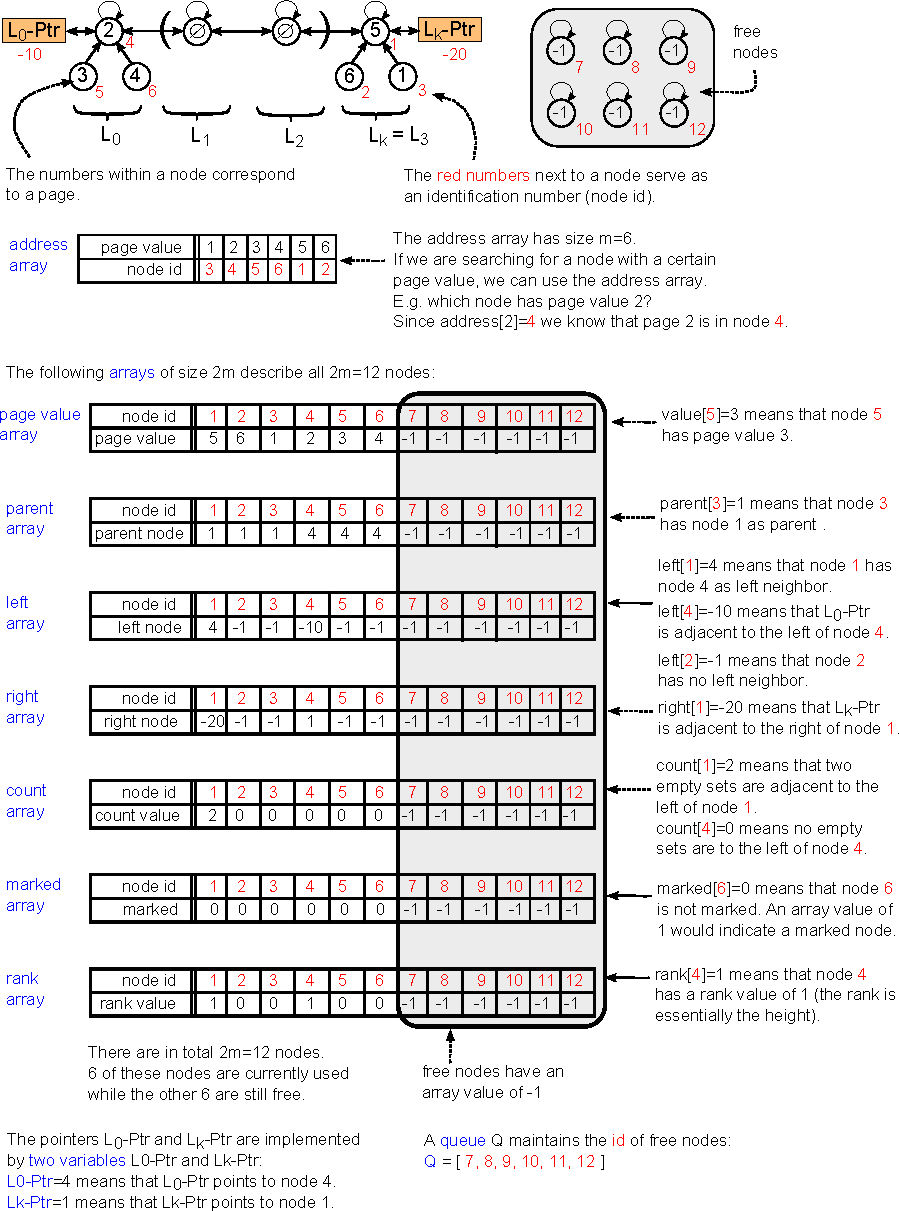
\includegraphics[scale=0.95]{./figures/java_implementation1.pdf}
	\caption{Implementation of LTrees in Java using arrays, two variables and a queue.} 
	\label{fig:java_implementation1}
\end{figure}

\noindent Each node has a \emph{page} value, a \emph{parent} pointer, a \emph{left} and \emph{right} pointer, a \emph{count} value, 
a \emph{marked} value and a \emph{rank} value. 
Each of these attributes is represented by an array of size $2m$ since there are in total $2m$ nodes. 
Two variables are used for the pointers $\cl_0$-Ptr and $\cl_k$-Ptr. A queue maintains which of the $2m$ nodes are still free.

Let us request page~3 to see how the arrays and queue are updated. The layer partition becomes 
$( \cl_0 | \cl_1 | \cl_2 | \cl_3) = (2,4 | \emptyset | 5,6,1 | 3)$, see figure~\ref{fig:java_implementation2}.

% figure: java_implementation2
\begin{figure}[htp]
	\centering
	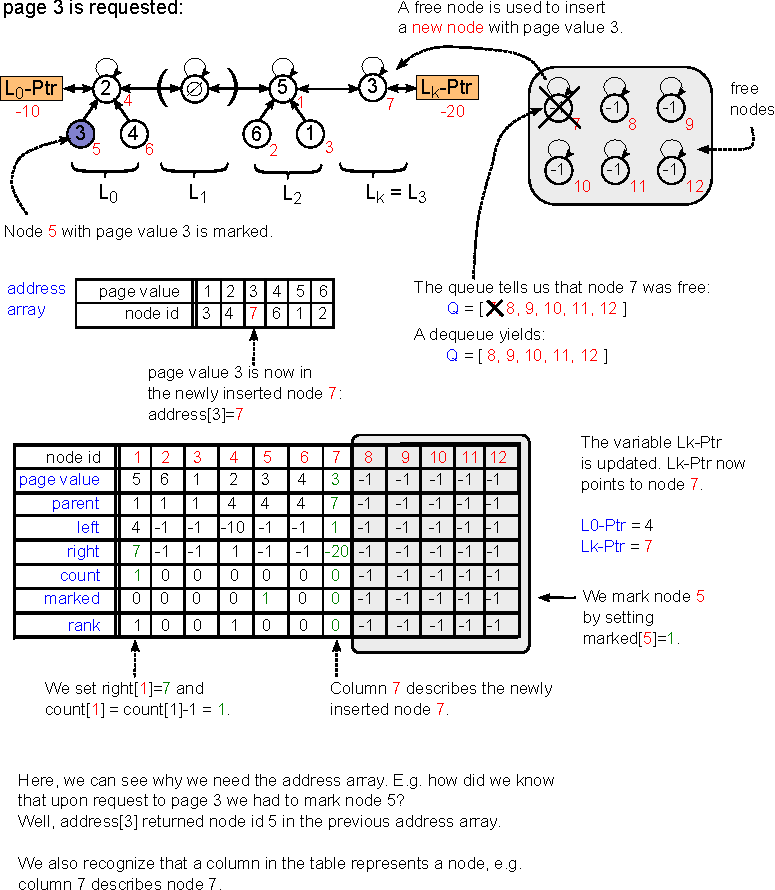
\includegraphics[scale=0.95]{./figures/java_implementation2.pdf}
	\caption{Implementation of LTrees in Java. The arrays, pointer variables and queue are updated upon request to page 3.} 
	\label{fig:java_implementation2}
\end{figure}

\noindent \textbf{Example 2}: Let us have a further look at the mechanics of LTrees, in particular 
at the cleanup procedure. Suppose the layer partition is given by 
$( \cl_0 | \cl_1 | \cl_2 | \cl_3) = (3,2 | \emptyset | 4,6,1 | 5)$ which we get after the request 
sequence $\sigma = (5,6,1,3,2,4,6,1,5)$. In figure~\ref{fig:java_implementation3} we see how LTrees looks like after the
last request (page 5). Note that the queue becomes empty indicating that no free nodes are available. 

% figure: java_implementation3
\begin{figure}[htp]
	\centering
	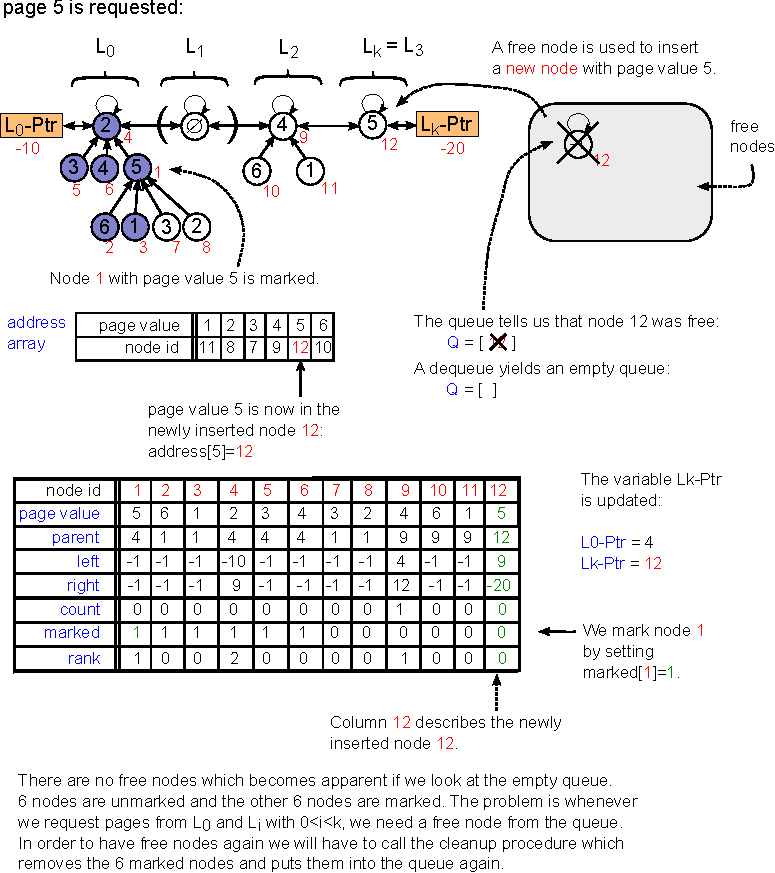
\includegraphics[scale=0.95]{./figures/java_implementation3.pdf}
	\caption{Implementation of LTrees in Java. The arrays, pointer variables and queue are updated upon request to page 5.
                    Note that the queue becomes empty.} 
	\label{fig:java_implementation3}
\end{figure}
 
\noindent \textbf{Example 3}: We have just seen that the queue is empty which means that all $2m=12$ nodes
are used in the linked trees data structure. The problem is whenever we request pages from $\cl_0$ and $\cl_i$ with $0<i<k$, 
we need a free node from the queue. In order to have free nodes again we will have to call the cleanup procedure which 
removes the $m=6$ marked nodes and puts them into the queue again. In step 1 of the cleanup procedure we apply a
find operation \emph{with path compression} to all $2m=12$ nodes which creates trees with height of at most 1, see figure~\ref{fig:java_implementation4}.

% figure: java_implementation4
\begin{figure}[htp]
	\centering
	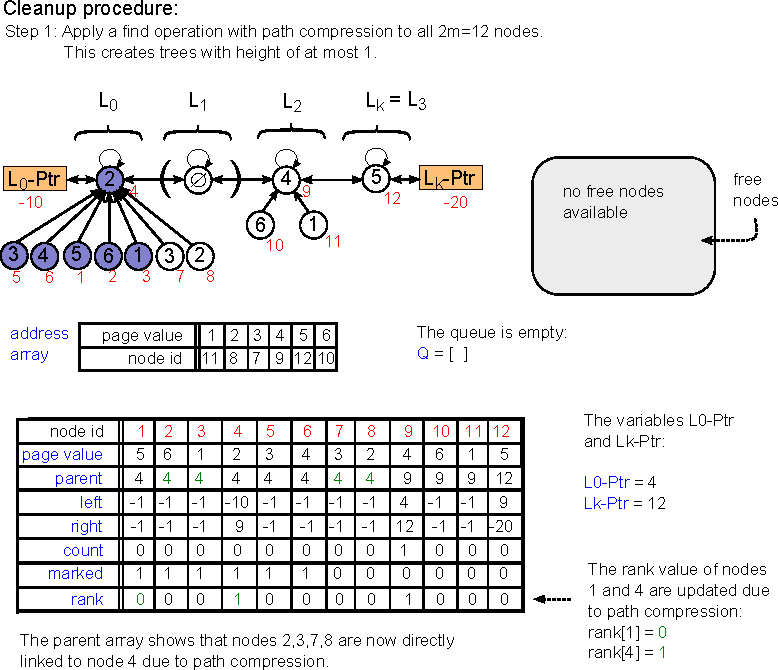
\includegraphics[scale=0.95]{./figures/java_implementation4.pdf}
	\caption{Step~1 of the cleanup procedure. A find operation with path compression is applied to all $2m$ nodes. 
                    This creates trees with height of at most 1. The parent and rank array are updated. Note that the rank
                    is only updated during the cleanup procedure, but usually it is not changed as mentioned in~\cite{brPreiss_onlineBook}.} 
	\label{fig:java_implementation4}
\end{figure}

\noindent Let us examine step 2 of the cleanup procedure where we remove marked nodes. 
In 2a) this is done for non-root nodes. The queue is filled with the id of these nodes, 
see figure~\ref{fig:java_implementation5}.

In 2b) marked root nodes are replaced by one of their children, see figure~\ref{fig:java_implementation6}.
After this step all previously marked nodes have been removed and free nodes are available again in the queue. 
Requesting pages is possible again.

% figure: java_implementation5
\begin{figure}[htp]
	\centering
	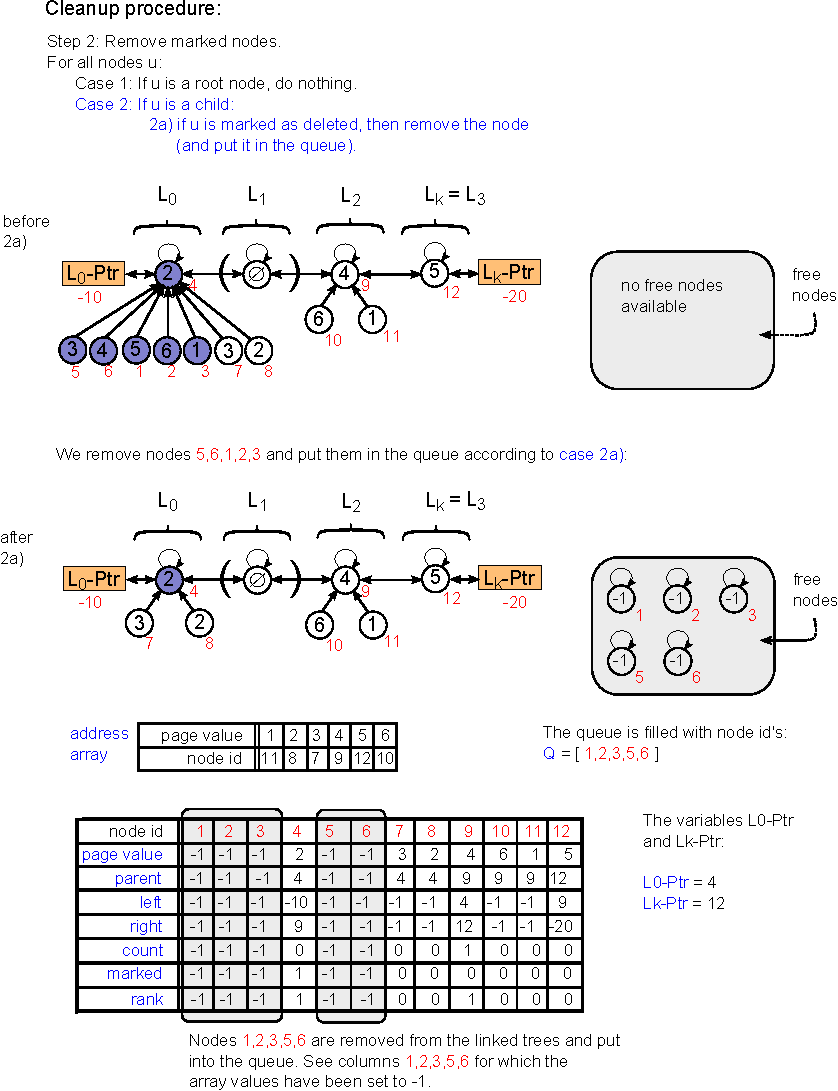
\includegraphics[scale=0.95]{./figures/java_implementation5.pdf}
	\caption{Step~2, case 2a) of the cleanup procedure. Marked nodes (non-root nodes) are removed and put into the queue.} 
	\label{fig:java_implementation5}
\end{figure}



% figure: java_implementation6
\begin{figure}[htp]
	\centering
	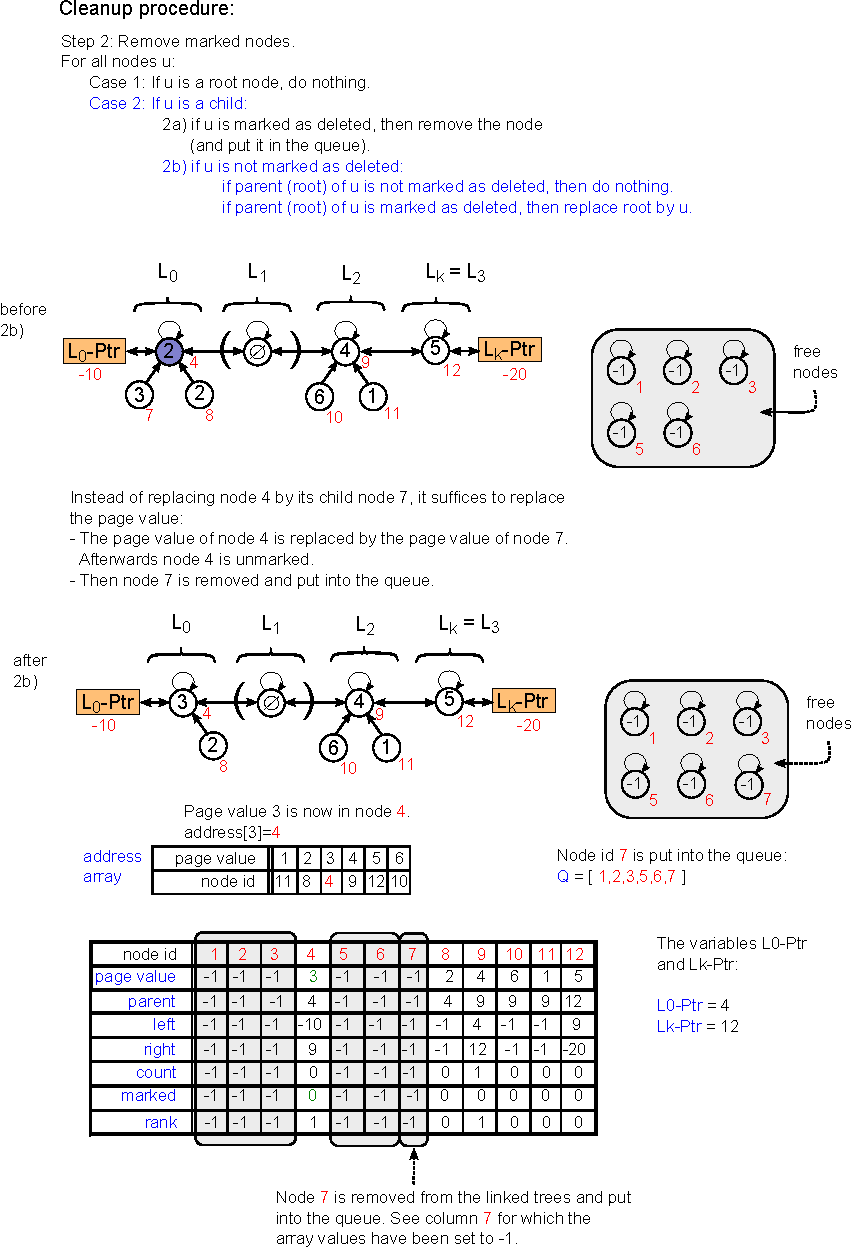
\includegraphics[scale=0.95]{./figures/java_implementation6.pdf}
	\caption{Step~2, case 2b) of the cleanup procedure. Marked root nodes are replaced by their children.} 
	\label{fig:java_implementation6}
\end{figure}


% subsection -----------------------------------------------------------------------------------
\subsection{Timestamp implementation of the layer partition}
Another possibility to implement the layer partition and therefore OPT is to use a timestamp based data structure
which we will refer to as \emph{TStamp}. It has been devised by Moruz et al.~\cite{sea12_paper}. 
Each layer $\cl_i$ is represented by a tuple $(t,v)$ where $t$ is the time of the 
layer creation. $t$ remains unchanged until $\cl_i$ is merged with $\cl_0$. The variable $v$ is defined as $v:=1+e$, where
$e$ is the number of empty layers adjacent to the left (this is similar to the count variable in LTrees). 
The layer $\cl_0$ is not stored by TStamp. 

%It is important to mention that TStamp can determine effectively in which particular layer $\cl_i$ a page $p$ is, 
%i.e. if $p \in \cl_i$, then the index $i$ can be found effectively in contrast to LTrees. \\
Moreover, TStamp stores information about when each page has last been requested. \\
\\
\textbf{Example 1}: Suppose we have the request sequence $\sigma=(5,6,1,3,2,4,5)$, 
a cache size of $k=3$ and the page-set $M=\{1,2,3,4,5,6\}$. The pages in $\sigma$ are requested at time $t$, 
see table~\ref{tab:timestamps}.

\begin{table}[htp]
\begin{center}
	\begin{tabular}{|c||c|c|c|c|c|c|c|}
	  	\hline
		pages in $\sigma$ & 5 & 6 & 1 & 3 & 2 & 4 & 5\\
		\hline		
		time $t$               & 1 & 2 & 3 & 4 & 5 & 6 & 7\\
		\hline
	\end{tabular}
	\caption{The pages in $\sigma$ are requested at time $t$.}
        \label{tab:timestamps}
\end{center}
\end{table}

\noindent \textbf{Request first three pages}: The layer partition after the first $k=3$ pairwise distinct requested pages is given in figure~\ref{fig:TStamp_layerPartition}.
Notice that we have added a line that states for each layer when it was created (except for the empty layers and $\cl_0$ which
are ignored), e.g. $\cl_3$ was created when page~5 was requested at time $t=1$. 

By layer creation we mean case $p \in \cl_0$ of the update rules for the layer partition, since $\cl_k$ will only contain
page $p$ such that $\cl_k = \{p\}$ can be considered as newly created layer. The other case is the first request in $\sigma$. 

% figure: TSTamp_layerPartition
\begin{figure}[htp]
	\centering
	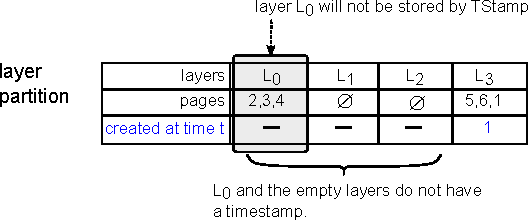
\includegraphics[scale=0.95]{./figures/TStamp_layerPartition.pdf}
	\caption{The layer partition after the first $k=3$ pairwise distinct requested pages. The third
                     row shows the time of the layer creation. } 
	\label{fig:TStamp_layerPartition}
\end{figure}

\noindent How does TStamp store the layer partition? TStamp encodes it in an array \emph{birth} with tuples $(t,v)$, 
see figure~\ref{fig:TStamp_birthArray}. 
The name birth indicates that $t$ describes the time when a layer was created. Its size is $k$ because at most 
$k$ layers, namely $\cl_1$ to $\cl_k$, are stored ($\cl_0$ is not stored).

% figure: TSTamp_birthArray
\begin{figure}[htp]
	\centering
	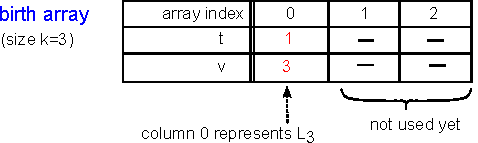
\includegraphics[scale=1.0]{./figures/TStamp_birthArray.pdf}
	\caption{TStamp encodes the layer partition in an array called birth. Its entries are tuples $(t,v)$.} 
	\label{fig:TStamp_birthArray}
\end{figure}

\noindent Layer $\cl_3$ is represented by column 0 which contains the tuple $(t,v)=(1,3)$. This means that 
$\cl_3$ has been created at time $t=1$, and its value for $v:=e+1$ equals 3 since $e=2$ empty layers 
are adjacent to the left. 

Moreover, TStamp keeps an array \emph{lastRequest} that assigns to each page the time of its last request, 
see figure~\ref{fig:TStamp_lastRequest}.

% figure: TSTamp_lastRequest
\begin{figure}[htp]
	\centering
	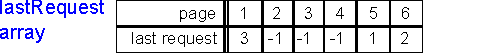
\includegraphics[scale=1.0]{./figures/TStamp_lastRequest.pdf}
	\caption{The array lastRequest after the first 3 requests. For each page the time of its last request is stored. 
                     The value -1 indicates that a page has not been requested yet.} 
	\label{fig:TStamp_lastRequest}
\end{figure}

\noindent \textbf{Request(3)}: Let us process the next request which is page~$3\in \cl_0$ at time $t=4$. The updated 
layer partition is shown in figure~\ref{fig:TStamp_layerPartition_t4}.

% figure: TSTamp_layerPartition_t4
\begin{figure}[htp]
	\centering
	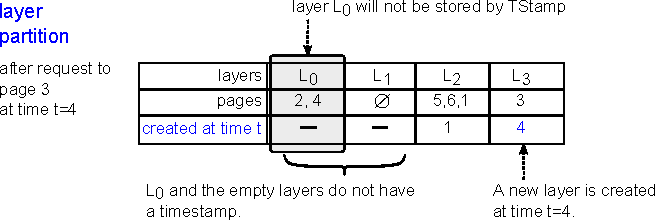
\includegraphics[scale=1.0]{./figures/TStamp_layerPartition_t4.pdf}
	\caption{The layer partition after request to page~3 at time $t=4$.} 
	\label{fig:TStamp_layerPartition_t4}
\end{figure}

\noindent A new layer is created at time $t=4$ such that we have to update the birth array, 
see figure~\ref{fig:TStamp_birthArray_t4}.
% figure: TSTamp_birthArray_t4
\begin{figure}[htp]
	\centering
	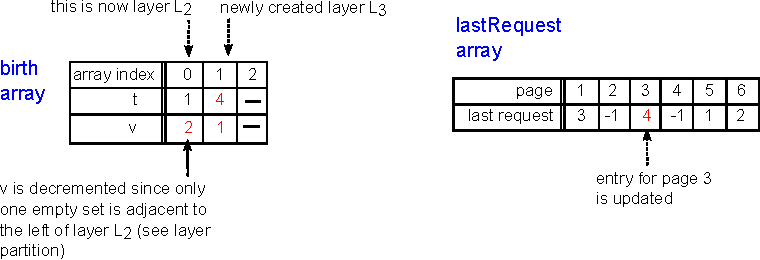
\includegraphics[scale=1.0]{./figures/TStamp_birthArray_t4.pdf}
	\caption{TStamp uses the two arrays birth and lastRequest. birth is updated because a new layer is created at time $t=4$.} 
	\label{fig:TStamp_birthArray_t4}
\end{figure}
The content of the birth array tells us that there are two non-empty layers. The first one with $(t,v)=(1,2)$ has been created
at time $t=1$ and has $e=v-1=1$ empty set adjacent to the left. 
The second one with $(t,v)=(4,1)$ has been created at time $t=4$ and has $e=v-1=0$ empty layers
adjacent to the left. We recognize that this is indeed the case for the layer partition in figure~\ref{fig:TStamp_layerPartition_t4}.\\
\\
\noindent \textbf{Request(2)}: We process the next request which is page~$2\in \cl_0$ at time $t=5$. 
The updated layer partition is shown in figure~\ref{fig:TStamp_request_t5}.
% figure: TSTamp_request_t5 with layer partition, birth array and lastRequest array --------------------------------------------------------
\begin{figure}[htp]
	\centering
	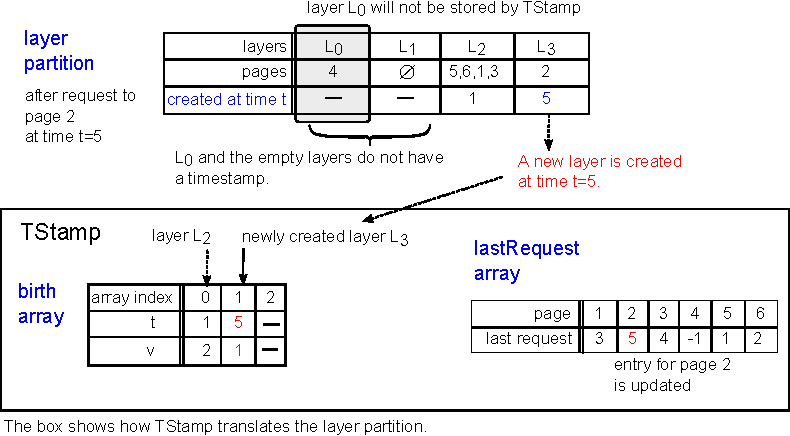
\includegraphics[scale=1.0]{./figures/TStamp_request_t5.pdf}
	\caption{The layer partition, birth array and lastRequest array upon request to page~2 at time $t=5$.
                     We recognize that the birth array encodes the structure of the layer partition.} 
	\label{fig:TStamp_request_t5}
\end{figure}

\newpage
\noindent \textbf{Request(4)}: We request page~$4\in \cl_0$ at time $t=6$, see figure~\ref{fig:TStamp_request_t6}.
% figure: TSTamp_request_t6 with layer partition, birth array and lastRequest array----------------------------------------------------------
\begin{figure}[htp]
	\centering
	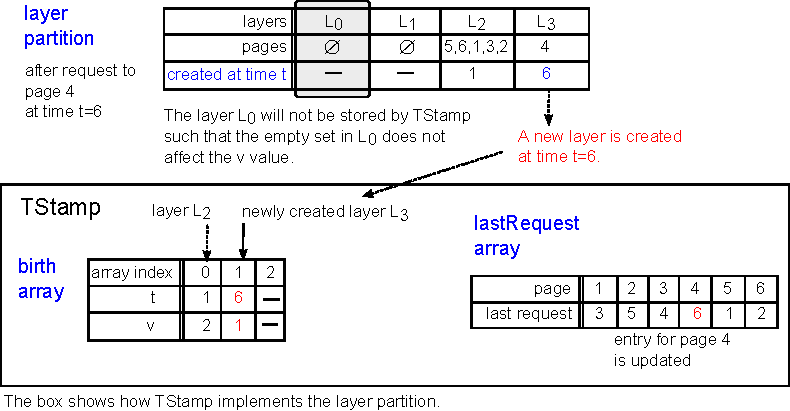
\includegraphics[scale=0.95]{./figures/TStamp_request_t6.pdf}
	\caption{The layer partition and TStamp at time $t=6$.} 
	\label{fig:TStamp_request_t6}
\end{figure}

\noindent \textbf{Request(5)}: We request page~$5\in \cl_2$ at time $t=7$, see figure~\ref{fig:TStamp_request_t7}.
% figure: TSTamp_request_t7 with layer partition, birth array and lastRequest array----------------------------------------------------------
\begin{figure}[htp]
	\centering
	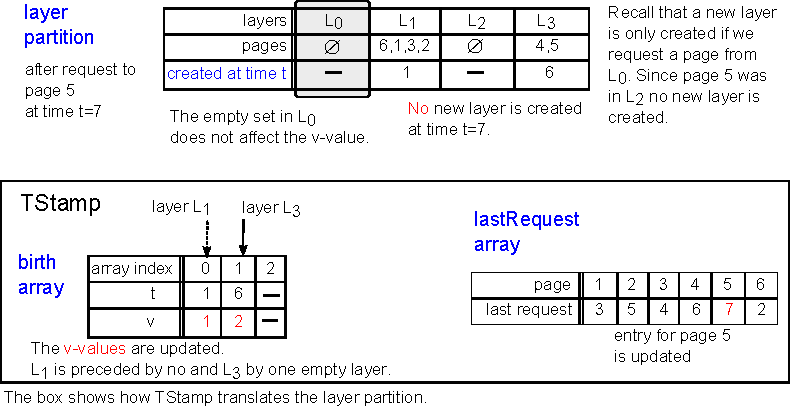
\includegraphics[scale=0.95]{./figures/TStamp_request_t7.pdf}
	\caption{The layer partition and TStamp at time $t=7$.} 
	\label{fig:TStamp_request_t7}
\end{figure}

\noindent Until now we have not mentioned how we can fully reconstruct the layer partition from the
birth and lastRequest array, in particular how the index $i$ is determined for a page $p \in \cl_i$.
For this purpose we will introduce a \emph{prefix sum} of $v$, see figure~\ref{fig:TStamp_prefixSum}.
We recognize that the prefix sum represents the index $i$ for a layer $\cl_i$! 
% figure: TSTamp_prefixSum  ----------------------------------------------------------
\begin{figure}[htp]
	\centering
	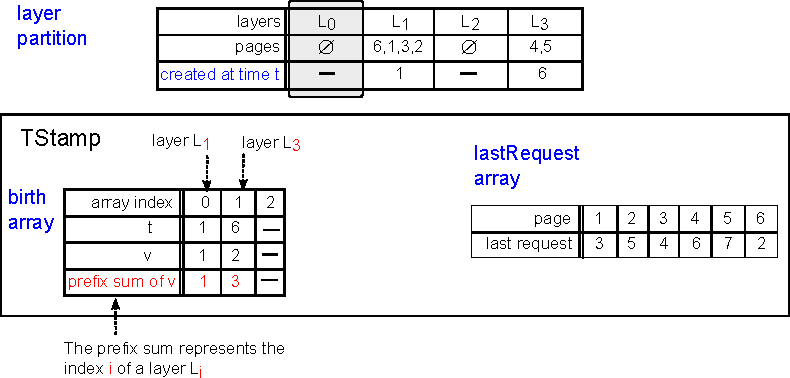
\includegraphics[scale=1.0]{./figures/TStamp_prefixSum.pdf}
	\caption{The birth array is extended by a prefix sum of $v$. The prefix sum corresponds to the index $i$ of a layer $\cl_i$.} 
	\label{fig:TStamp_prefixSum}
\end{figure}
As an example we will determine in which
layer page~3 is. In figure~\ref{fig:TStamp_prefixSum} we will walk along the birth array from right to left and ask some questions:

We are at array index~1 of the birth array: can page~3 be in $\cl_3$? No, it can't since page~3 has last been requested
at time $t=4$ but $\cl_3$ has been
created at time $t=6$. A page should have been requested at time $t \geq 6$ to be in $\cl_3$ which is not the case
for page~3.

We notice that the $t$ values in the birth array decrease if we go from right to left, i.e. for two layers
$\cl_i$ and $\cl_j$ with $i<j$ created at time $\cl_i.t$ and $\cl_j.t$ respectively we have $\cl_i.t < \cl_j.t$.
For example, we can see that $\cl_1.t < \cl_3.t$ with $\cl_1.t=1$ and $\cl_3.t=6$. 

We move one position to the left in the birth array, i.e. to array index~0, and ask: 
can page~3 be in $\cl_1$? Yes, it can since page~3 has last been requested at time $t=4$ and layer $\cl_1$ has been 
created at time $t=1$. The idea is that for a page $p$ to be in layer $\cl_i$ the following must hold\footnote{The concept 
is similar to the \emph{table of contents} in a book. 
We can easily determine in which chapter we are by looking at the page numbers of the chapter headings.}:

\[
\text{lastRequest[$p$]} \geq \cl_i.t
\]

\noindent To determine $\cl_i$ we move along the birth array from right to left, and as soon
as the condition above is fulfilled we have found $\cl_i$. 
Let us illustrate this for page~6. Once again we move from right to left in the birth array:

- Is $6 \in \cl_3$? No, since lastRequest[6] $< \cl_3.t$. 

- Is $6 \in \cl_1$? Yes, since lastRequest[6] $\geq \cl_1.t$.


\newpage
\noindent \textbf{Example 2:} Suppose the cache size is $k=3$, the page-set $M=\{1,2,3,4,5,6\}$ 
and the layer partition is given by $( \cl_0 | \cl_1 | \cl_2 | \cl_3) = (3 | 4,6 | 1,5 | 2)$, see figure~\ref{fig:TStamp_prefixSum2}.

% figure: TSTamp_prefixSum2  ----------------------------------------------------------
\begin{figure}[htp]
	\centering
	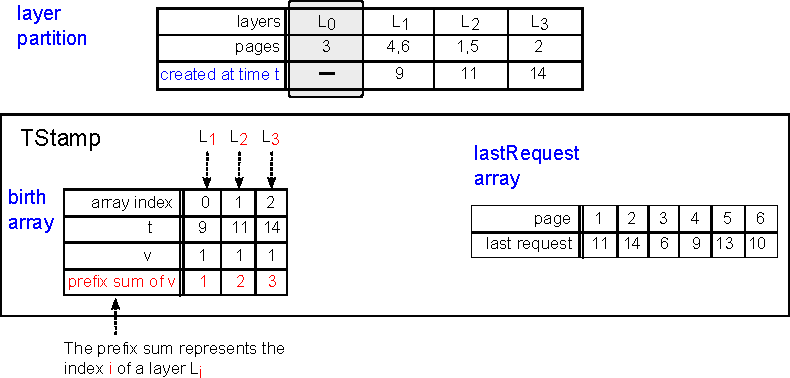
\includegraphics[scale=1.0]{./figures/TStamp_prefixSum2.pdf}
	\caption{TStamp implementation of the layer partition in example 2.} 
	\label{fig:TStamp_prefixSum2}
\end{figure}

\noindent We will determine in which layer page~3 is by looking only at birth and lastRequest.
The prefix sum tells us the layer index. Once again we move from right to left in the birth array:

- Is $3 \in \cl_3$? No, since lastRequest[3]$<\cl_3.t$.

- Is $3 \in \cl_2$? No, since lastRequest[3]$<\cl_2.t$.

- Is $3 \in \cl_1$? No, since lastRequest[3]$<\cl_1.t$.

\noindent We cannot move further to the left in birth which means that $3\in \cl_0$.\\
\\
\noindent Let us determine in which layer page~2 is. Moving from right to left in the birth array we ask:

- Is $2\in \cl_3$? Yes, since lastRequest[2]$\geq \cl_3.t$.

\noindent Note that instead of moving from right to left in the birth array we can also use binary search.\\
\\
\noindent \textbf{Update rules upon a page request}\\
Recall that upon a request to page $p$ the layer partition is modified according to three update rules (see again section~\ref{sec:LayerPartition}), 
and in the previous examples we have seen how the cases $p \in \cl_0$ and $p \in \cl_i$ with $0<i<k$ are handled by TStamp.
We want to formalize how TStamp translates the update rules:

\begin{itemize}
   \item Case (i): If $p \in \cl_0$, then $\cl_k$ is merged into $\cl_{k-1}$. Afterwards, $p$ is removed from
    $\cl_0$ and inserted as new layer $\cl'_k$ such that $\cl'_k=\{p\}$.
        
	Merging $\cl_k$ with $\cl_{k-1}$ is done as follows: 
        if $\cl_{k-1}$ is empty, then the $v$ value for $\cl_{k}$ is decremented since the number of empty layers to the left of $\cl_k$ 
        decreases by one. Then we append a new column in the birth array with a tuple $(t,v)$, where $t$ is the current timestamp
        and $v=1$. This column represents the new layer $\cl'_k$ (see figure~\ref{fig:TStamp_birthArray_t4}).
  
	Otherwise, if $\cl_{k-1}$ is not empty, then we simply overwrite the $t$ value for $\cl_{k}$ by the current
        timestamp\footnote{
	If you think of the \emph{table of contents analogy}, then this corresponds to putting the last chapter heading to the very end of a book.}
        (see figure~\ref{fig:TStamp_request_t5}).

        Finally, we set lastRequest[$p$] to the current timestamp such that the new last layer $\cl'_k$ contains only $p$.          
   \item Case (ii) If $p \in \cl_k$, then the layer partition remains the same. Therefore, TStamp does not need to be updated.
   \item Case (iii): If $p \in \cl_i$ with $0<i<k$, then $p$ is removed from $\cl_i$ and added to $\cl_k$.
            Afterwards $\cl_i \backslash \{p\}$ is merged into $\cl_{i-1}$. The layers $\cl_j$ with $j=i+1,i+2,\dots,k-1$ all move one position to the left. 
           An empty set is inserted as new layer $\cl'_{k-1}$ such that $\cl'_{k-1}=\emptyset$.

           In order to move $p$ from $\cl_i$ to $\cl_k$ we set lastRequest[$p$] to the current timestamp. 

	Merging $\cl_i \backslash \{p\}$ with 
           $\cl_{i-1}$ and shifting layers $\cl_j$ with $j=i+1,i+2,\dots,k-1$ one position to the left is done as follows: if $\cl_{i-1}$ is empty, 
           then the $v$ value for $\cl_i$ is decremented (see figure~\ref{fig:TStamp_request_t7}). 
	   
	   Otherwise, if $\cl_{i-1}$ is not empty, then we delete the column for $\cl_i$ in the birth array and move all the following columns 
           one position to the left (see figure~\ref{fig:TStamp_deleteLayer}). 

	   Finally, to insert an empty set as new layer $\cl'_{k-1}$ we simply increment the $v$ value for $\cl_k$. 	

\end{itemize} 


\subsubsection{Runtime analysis for TStamp}
\label{sec:runtimeAnalysisTStamp}
Cases (i) and (ii) are handled by TStamp in $\oh(1)$ time. 
In case (iii) however, processing a request to page $p \in \cl_i$ with $0<i<k$ can be slow for TStamp as shown in figure~\ref{fig:TStamp_deleteLayer}:
an update of the layer partition involves merging two layers.   
TStamp implements this union of two layers by deleting an entry in the birth array. In the worst case 
this is the first entry such that all $k-1$ following entries have to be shifted one position to 
the left which requires $\oh(k)$ time.\\
\\
\noindent \textbf{Remark (R1)}: The worst-case time is $\oh(k)$, but we should consider the following:
although the birth array has size $k$ deleting the first column can still be fast. The reason 
is that the birth array is not necessarily filled with $k$ columns. For example, in figure~\ref{fig:TStamp_prefixSum}
you can see that the last column of the birth array is not occupied since out of the three layers $\cl_1, \cl_2$ and $\cl_3$ 
only the two non-empty layers $\cl_1$ and $\cl_3$ are stored as columns.  

Or consider this example: if $k=2000$, then there may only be 10 non-empty layers such 
that only 10 columns are occupied in the birth array. In that case deleting the first column implies
shifting only 9 columns instead of $k-1=1999$ columns. 

If $l$ is the number of non-empty layers, then $l-1$ columns have to be shifted to the left, 
and processing a page request then requires $\oh(l)$ time. 
Moruz et al.~\cite{sea12_paper} examined how TStamp processes some real-world traces. 
They showed empirically that $l$ is a small number, i.e. there are significantly less than $k$ non-empty layers. 

Moreover, a page that is requested from $\cl_k$ is processed by TStamp in $\oh(1)$ time, and 
for the traces examined by Moruz et al.  99\% of the requested pages are from $\cl_k$.\\
\\
\noindent \textbf{Proposition 2}: If $p \in \cl_0$ or $p \in \cl_k$, then TStamp processes a request to page $p$ in $\oh(1)$ time. 
If $p \in \cl_i$ with $0<i<k$, then TStamp requires $\oh(l)$ time with $l$ being the number of non-empty layers. 
The worst-case time is $\oh(k)$.

% figure: TSTamp_deleteLayer  ----------------------------------------------------------
\begin{figure}[htp]
	\centering
	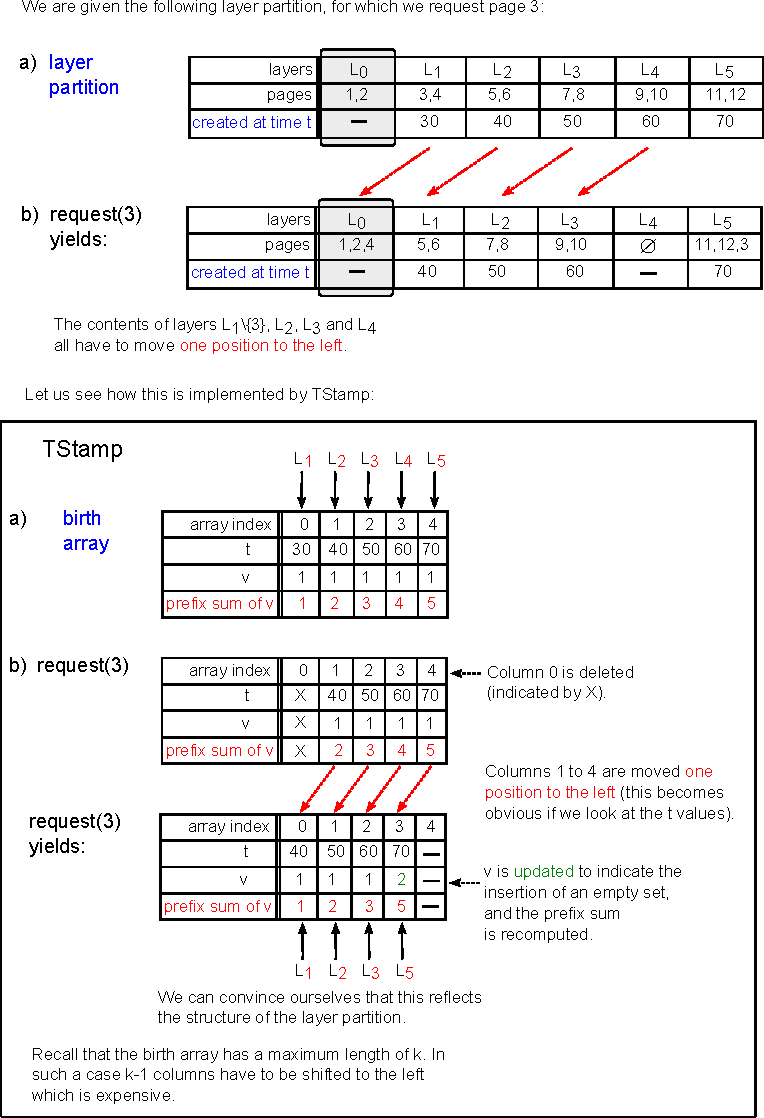
\includegraphics[scale=1.0]{./figures/TStamp_deleteLayer.pdf}
	\caption{Page~$3 \in \cl_1$ is requested. TStamp merges $\cl_1 \backslash \{3\}$ with $\cl_0$ by deleting the first column in the birth array
                     and shifting all the following columns one position to the left.} 
	\label{fig:TStamp_deleteLayer}
\end{figure}



\subsubsection{Space requirements for TStamp}
TStamp stores the arrays birth and lastRequest. The birth array has size $k$ and the lastRequest array size $m$. 
Since $m \geq k$ the total space required by TStamp is $\theta(m)$.

\newpage
\subsection{Comparison of LTrees and TStamp}
We want to compare some features of LTrees and TStamp, where
$k$ is the cache size and $m$ the page-set size, see table~\ref{tab:comparison}.
%E.g. TStamp only needs $\oh(\log(k))$ time to find the index $i$ for a page $p\in \cl_i$
%via a binary search.
%By comparison LTrees achieves this as follows: 
%in LTrees we first apply a find($p$) operation which returns the root node $r$ in $\oh(\alpha(2m))$ time.
%From $r$ we follow the left pointers and count the number of layers we traverse (including the empty layers) until we reach the root node of $\cl_0$,
%which requires $\oh(k)$ time. This gives us the value for $i$ in $\oh( \alpha(2m) + k)$ time.
It is not clear which of the data structures has the better runtime when processing a request sequence $\sigma$.
For this reason we we will compare their runtimes experimentally for five real-world traces in the next section.


\begin{table}[hb]
\begin{center}
	\begin{tabular}{|l||l|l|}
	  	\hline
		                                 &        LTrees                                      &   TStamp                  \\
		\hline  
		process request   &        $\oh(1)$ for $p \in \cl_k$,                  & $\oh(1)$ for $p \in \cl_k$,                 \\
                 to page $p$        &	    $\oh( \alpha(2m))$ amortized              & $\oh(1)$ for $p \in \cl_0$,                 \\      
                                          &        for $p \in \cl_0$  and                          & $\oh(l)$ for $p \in \cl_i$ with  $0<i<k$ \\
                                          &        $p \in \cl_i$ with  $0<i<k$                  & and $l$ non-empty layers, \\
                                         &                                                                 &  $\oh(k)$ worst-case                    \\
		\hline
%                find index layer $i$      &	   $\oh( \alpha(2m) +k )$                &  $\oh(\log(k))$      \\
%		for $p \in \cl_i$           &                                                         &                                                    \\                
%		\hline
		space                       &          $\theta(m)$                              &  $\theta(m)$  \\     
                \hline
	\end{tabular}
	\caption{Comparison of the data structures LTrees and TStamp. 
                     $k$ is the cache size and $m$ the page-set size.}
        \label{tab:comparison}
\end{center}
\end{table}

\subsubsection{Borrowing a technique from TStamp}
Before we present the experimental results we will modify LTrees a little by borrowing a technique
from TStamp. Upon a request to page~$p$ the case $p \in \cl_k$ can be recognized by TStamp very quickly in $\oh(1)$ time by
comparing lastRequest[$p$] with the time $\cl_k.t$ that states when 
$\cl_k$ was created. If lastRequest[$p$]$\geq \cl_k.t$, then $p$ is in layer $\cl_k$.

For LTrees we will adopt the lastRequest array and introduce a variable $t_0$ that stores 
the time when $\cl_k$ was created (which is also the time when we have last requested a page from $\cl_0$). 
Similar to TStamp we check if lastRequest[$p$]$\geq t_0$ to recognize the case $p \in \cl_k$. 

Although LTrees processes the case $p \in \cl_k$ in $\oh(1)$ anyway since the tree for $\cl_k$ 
has always height of at most 1, we found that this technique improves the runtime 
of LTrees in the experiments.

 

% EXPERIMENTS
\newpage
\section{Experiments}

\subsection{Setup}

In this section the runtimes of LTrees and TStamp are compared for the traces in table~\ref{tab:traces}.
The traces, which can be found in~\cite{arc_paper}, represent long request sequences and have been 
obtained from real-world applications.



\begin{table}[hb]
\begin{center}
	\begin{tabular}{|r||r|r|}
	  	\hline
                trace name                              &     number of requests        &      unique pages \\
               (request sequence $\sigma$)     &     (length of $\sigma$)       &      (page-set size $m$) \\
		\hline
               OLTP                                       &          914,145                  &      186,880      \\
               \hline		
		S1                                          &       3,995,316                   &     1,309,698   \\
		\hline
                P6                                          &      12,672,123                   &      773,770     \\
                \hline
                P1                                          &      32,055,473                   &    2,311,485    \\
                \hline
               SPC1 like                                 &      41,351,279                  &      6,050,363   \\
                \hline
	\end{tabular}
	\caption{Traces with their features.}
        \label{tab:traces}
\end{center}
\end{table}

\noindent Two setups have been used:
\begin{itemize}
	\item Samsung notebook PC, Intel Atom processor @1.66 GHz, 1~GB RAM, Windows~7, Java~SE7
        \item Lenovo desktop PC, Intel Core i3-2100 CPU @3.1 GHz, 4~GB RAM, Windows~7, Java~SE6
\end{itemize}

The runtime for processing a trace was measured three times, and the median was chosen to compare 
LTrees with TStamp. Both data structures have been implemented in Java. 

For LTrees we had to increase the Java heap space, i.e. the memory available to Java, since
the traces have a large page-set size $m$, and LTrees uses several arrays of size $2m$.
In the Eclipse IDE the Java heap space can be changed via the argument -Xmx[space]. For the Samsung 
notebook PC we chose -Xmx550M and for the Lenovo desktop PC -Xmx1024M. 

Regarding the queue in LTrees the following was observed for the trace P6 
and a cache size $k=4096$ on the Samsung notebook PC: we have first used
the queue that is offered by the Java API for which there are several implementations. 
We started with the LinkedList implementation which lead to a runtime of 29 seconds. 
After some research~\cite{queue_stackoverflow} we used the faster ArrayDeque implementation which
processed the trace in 24 seconds. 
Note that the queue from the Java API is designed to store objects. 
However, the pages in the tracefile are represented by integers.
So we switched to a queue for primitive data types~\cite{queue_primitive} which improved the 
runtime to 20 seconds. 

\newpage
\subsection{Results}
The results are presented in a table and a corresponding plot. The table shows the runtimes 
when processing the trace file for different cache sizes $k$. Notice that $k$ is not determined
by the trace file but can be set by us. For $k$ we have chosen powers of 2 as described 
in~\cite{arc_paper}, i.e. $k \in \{1024, 2048,4096,8192, 16384,32768,65536,131072, 262144, 524288 \}$. An exception 
is trace OLTP where we chose $k \in \{1000,2000,5000,10000,15000\}$.
The purpose of the table is to demonstrate the behaviour of the data structure towards increasing cache sizes. 

To compare LTrees with TStamp the ratios of their runtimes are displayed in a plot for 
different cache sizes. Since $k$ increases in powers of two the $x$-axis is shown in a logarithmic scale. 
A red line at height 1 of the $y$-axis marks points of equal runtimes making it easier to recognize where 
each data structure performs better. Points below this line indicate a better performance for TStamp, whereas
points above this line mean a better performance for LTrees.


Table~\ref{tab:cacheMissesTraces} lists for each trace the number of cache misses performed by OPT.  
These values are obtained by counting the number of requested pages from layer $\cl_0$
(see again property (Pr1) in section~\ref{sec:LayerPartition}) and are equal for both LTrees
and TStamp since they both implement the layer partition. The values also include the first $k$ pairwise 
distinct requested pages which cause a cache miss since these pages have not been in the initially empty cache.


%OOOOOOOOOOOOOOOOOOOOOOOOOOOOOOOOOOOOOOOOOOOOOOOOOOOOOOOOOOOOOOO
% plot  ----------------------------------------------------------
\begin{figure}[p]
	\centering
	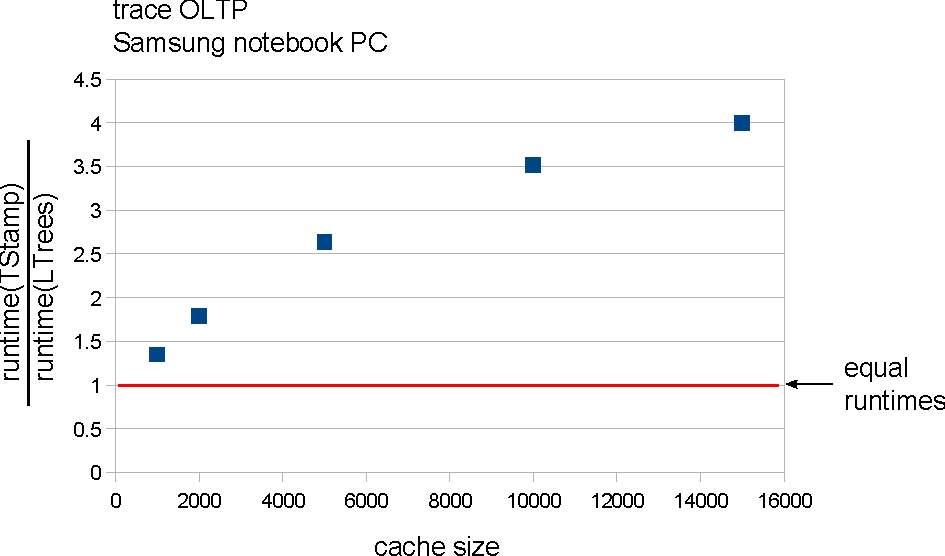
\includegraphics[scale=0.8]{./experiments/samsung_OLTP.pdf}
	\caption{The ratio runtime(TStamp)/runtime(LTrees) is plotted against the cache size.
                     The red line corresponds to points of equal runtimes.} 
	\label{fig:samsung_OLTP}
\end{figure}


% table ----------------------------------------------------------
\begin{table}[p]
\begin{center}
	trace OLTP processed on Samsung notebook PC
	\begin{tabular}{|r||r|r|r|}
	  	\hline
                cache size                               &     runtime LTrees         &      runtime TStamp          &  runtime(TStamp)/ \\
                                                             &      (in seconds)            &      (in seconds)                 & runtime(LTrees)     \\
                \hline
                1000			                     &         1.560                     &          2.106                          &      1.35            \\
		2000					     &         1.576                     &          2.823                          &      1.79            \\								
		5000					     &         1.607                     &          4.244                          &      2.64            \\	
		10000		         	     &         1.592                     &          5.601                          &      3.52            \\	
		15000				     &         1.544                     &          6.178                          &      4.00             \\	
		\hline
	\end{tabular}
	\caption{Results for the trace OLTP using the Samsung notebook PC. The trace was not processed on the Lenovo
                     desktop PC because the runtimes were too small and thus inaccurate.}
        \label{tab:samsung_OLTP}
\end{center}
\end{table}



% OOOOOOOOOOOOOOOOOOOOOOOOOOOOOOOOOOOOOOOOOOOOOOOOOOOOOOOO
% plot  ----------------------------------------------------------
\begin{figure}[p]
	\centering
	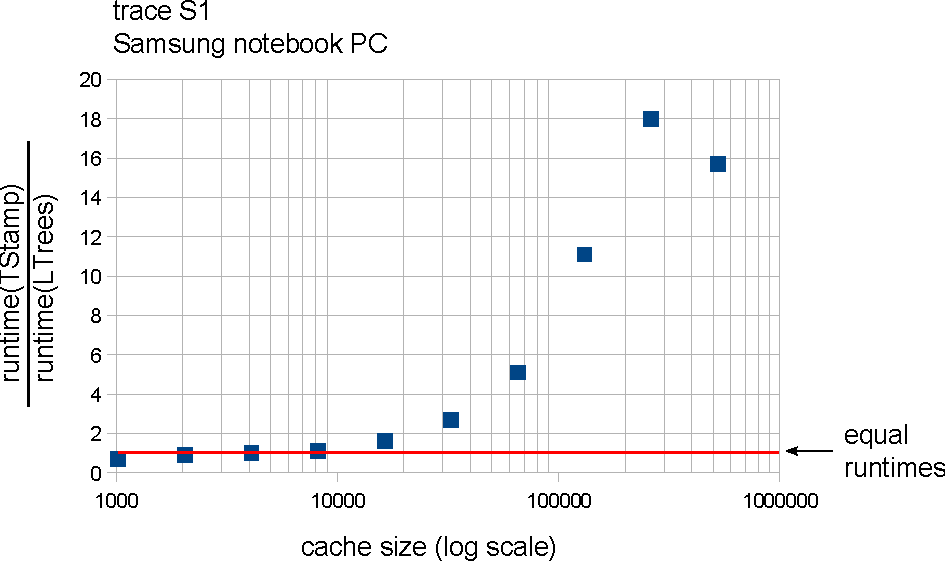
\includegraphics[scale=0.8]{./experiments/samsung_S1.pdf}
	\caption{The ratio runtime(TStamp)/runtime(LTrees) is plotted against the cache size.
                     The red line corresponds to points of equal runtimes.} 
	\label{fig:samsung_S1}
\end{figure}


% table ----------------------------------------------------------
\begin{table}[p]
\begin{center}
	trace S1 processed on Samsung notebook PC
	\begin{tabular}{|r||r|r|r|}
	  	\hline
                cache size                               &     runtime LTrees         &      runtime TStamp          &  runtime(TStamp)/ \\
                                                             &      (in seconds)            &      (in seconds)                 & runtime(LTrees)     \\
                \hline
                1024			             &            7                  &              5                      &        0.7                \\
		2048					     &              7                &        6                            &     0.9                   \\								
		4096					     &              7                &        7                            &     1.0                   \\	
		8192					     &              7                &        8                            &     1.1                   \\	
		16384				     &              7                &        11                            &    1.6                    \\	
		32768				     &              7                &        19                            &    2.7                    \\	
		65536				     &              7                &        36                            &    5.1                    \\	
		131072				     &              7                &        78                            &    11.1                    \\	
		262144				     &              7                &       126                             &   18.0                     \\	
		524288				     &              7                &       110                             &    15.7                    \\
                \hline
	\end{tabular}
	\caption{Results for the trace S1 using the Samsung notebook PC.}
        \label{tab:samsung_S1}
\end{center}
\end{table}



%OOOOOOOOOOOOOOOOOOOOOOOOOOOOOOOOOOOOOOOOOOOOOOOOOOOOOOOOOOOO
% plot  ----------------------------------------------------------
\begin{figure}[p]
	\centering
	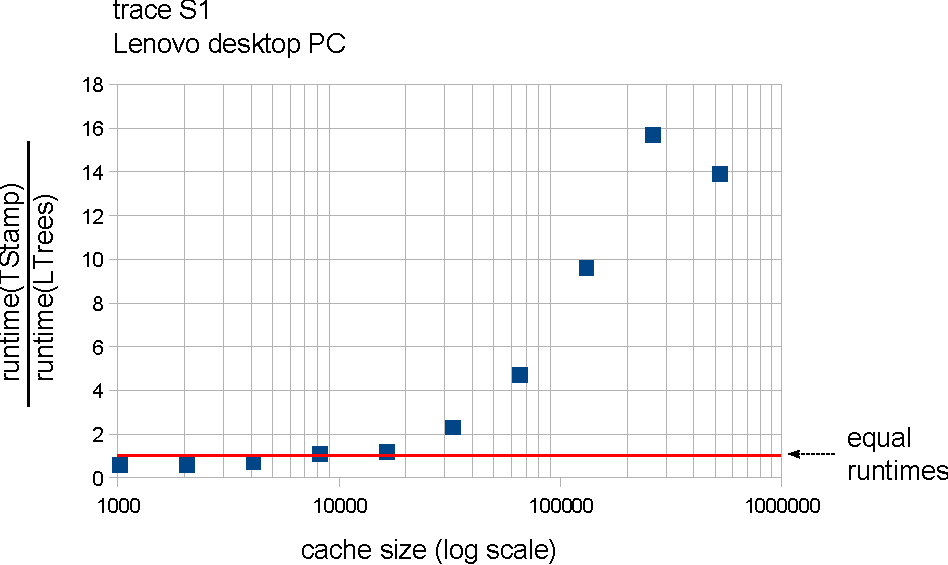
\includegraphics[scale=0.8]{./experiments/lenovo_S1.pdf}
	\caption{The ratio runtime(TStamp)/runtime(LTrees) is plotted against the cache size.
                     The red line corresponds to points of equal runtimes.} 
	\label{fig:lenovo_S1}
\end{figure}


% table ----------------------------------------------------------
\begin{table}[p]
\begin{center}
	trace S1 processed on Lenovo desktop PC
	\begin{tabular}{|r||r|r|r|}
	  	\hline
                cache size                               &     runtime LTrees         &      runtime TStamp          &  runtime(TStamp)/ \\
                                                             &      (in seconds)            &      (in seconds)                 & runtime(LTrees)     \\
                \hline
                1024			             &            1.092                  &            0.640                        &         0.59               \\
		2048					     &         1.076                     &    0.687                                &     0.64                   \\								
		4096					     &         1.092                     &     0.764                               &     0.70                   \\	
		8192					     &         1.123                     &     1.187                               &     1.06                   \\	
		16384				     &         1.139                     &     1.405                               &     1.23                   \\	
		32768				     &         1.154                     &     2.606                               &     2.26                   \\	
		65536				     &         1.124                     &     5.227                               &     4.65                   \\	
		131072				     &         1.140                     &      10.905                              &     9.57                   \\	
		262144				     &         1.124                     &    17.661                                &   15.71                     \\	
		524288				     &         1.117                     &     15.538                               &   13.91                     \\
                \hline
	\end{tabular}
	\caption{Results for the trace S1 using the Lenovo desktop PC.}
        \label{tab:lenovo_S1}
\end{center}
\end{table}



%OOOOOOOOOOOOOOOOOOOOOOOOOOOOOOOOOOOOOOOOOOOOOOOOOOOOOOOOOOOO
% plot  ----------------------------------------------------------
\begin{figure}[p]
	\centering
	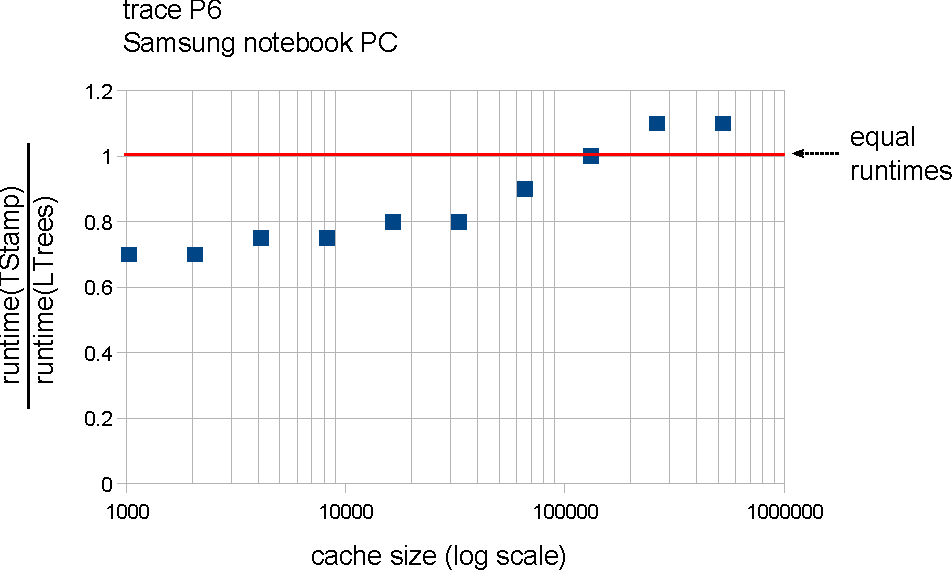
\includegraphics[scale=0.8]{./experiments/samsung_P6.pdf}
	\caption{The ratio runtime(TStamp)/runtime(LTrees) is plotted against the cache size.
                     The red line corresponds to points of equal runtimes.} 
	\label{fig:samsung_P6}
\end{figure}

% table ----------------------------------------------------------
\begin{table}[p]
\begin{center}
        trace P6 processed on Samsung notebook PC
	\begin{tabular}{|r||r|r|r|}
	  	\hline
                cache size                               &     runtime LTrees         &      runtime TStamp          &  runtime(TStamp)/ \\
                                                             &      (in seconds)            &      (in seconds)                 & runtime(LTrees)     \\
                \hline
                1024					     &         20                       &           14                            &       0.7                  \\
		2048					     &         20                       &           14                            &       0.7                      \\								
		4096					     &         20                       &           15                             &      0.75                       \\	
		8192					     &         20                       &           15                             &      0.75                       \\	
		16384				     &         19                       &           16                             &      0.8                       \\	
		32768				     &         19                       &           16                             &      0.8                       \\	
		65536				     &         18                      &            17                             &      0.9                       \\	
		131072				     &         17                      &            17                             &       1.0                      \\	
		262144				     &         17                      &            18                             &       1.1                      \\	
		524288				     &         16                      &            17                             &       1.1                      \\
                \hline
	\end{tabular}
	\caption{Results for the trace P6 using the Samsung notebook PC.}
        \label{tab:samsung_P6}
\end{center}
\end{table}



%OOOOOOOOOOOOOOOOOOOOOOOOOOOOOOOOOOOOOOOOOOOOOOOOOOOOOOOOOOOO
% plot  ----------------------------------------------------------
\begin{figure}[p]
	\centering
	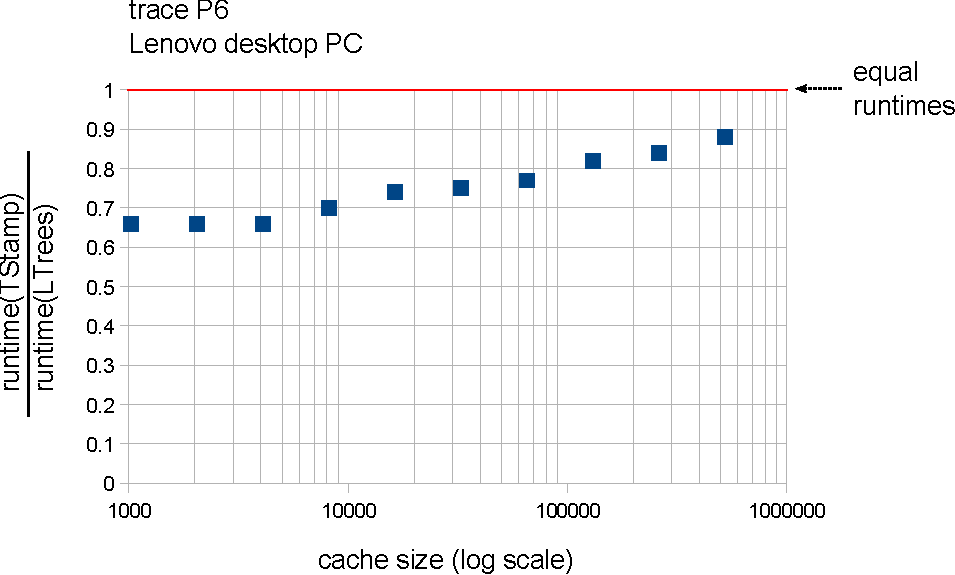
\includegraphics[scale=0.8]{./experiments/lenovo_P6.pdf}
	\caption{The ratio runtime(TStamp)/runtime(LTrees) is plotted against the cache size.
                     The red line corresponds to points of equal runtimes.} 
	\label{fig:lenovo_P6}
\end{figure}

% table ----------------------------------------------------------
\begin{table}[p]
\begin{center}
	trace P6 processed on Lenovo desktop PC
	\begin{tabular}{|r||r|r|r|}
	  	\hline
                cache size                               &     runtime LTrees         &      runtime TStamp          &  runtime(TStamp)/ \\
                                                             &      (in seconds)            &      (in seconds)                 & runtime(LTrees)     \\
                \hline
                1024					     &         2.122                  &           1.405                      &        0.66               \\
		2048					     &         2.138                  &           1.420                        &        0.66                \\								
		4096					     &         2.232                  &           1.468                         &     0.66                   \\	
		8192					     &         2.169                  &           1.514                         &     0.70                   \\	
		16384				     &        2.185                   &           1.623                         &     0.74                   \\	
		32768				     &        2.201                   &            1.655                        &     0.75                    \\	
		65536				     &        2.138                  &            1.654                        &      0.77                   \\	
		131072				     &        2.076                      &        1.702                            &  0.82                       \\	
		262144				     &        2.029                      &        1.701                            &  0.84                       \\	
		524288				     &        1.920                      &          1.686                          &    0.88                     \\
                \hline
	\end{tabular}
	\caption{Results for the trace P6 using the Lenovo desktop PC.}
        \label{tab:lenovo_P6}
\end{center}
\end{table}


%OOOOOOOOOOOOOOOOOOOOOOOOOOOOOOOOOOOOOOOOOOOOOOOOOOOOOOOOOOOOOOO
% plot  ----------------------------------------------------------
\begin{figure}[p]
	\centering
	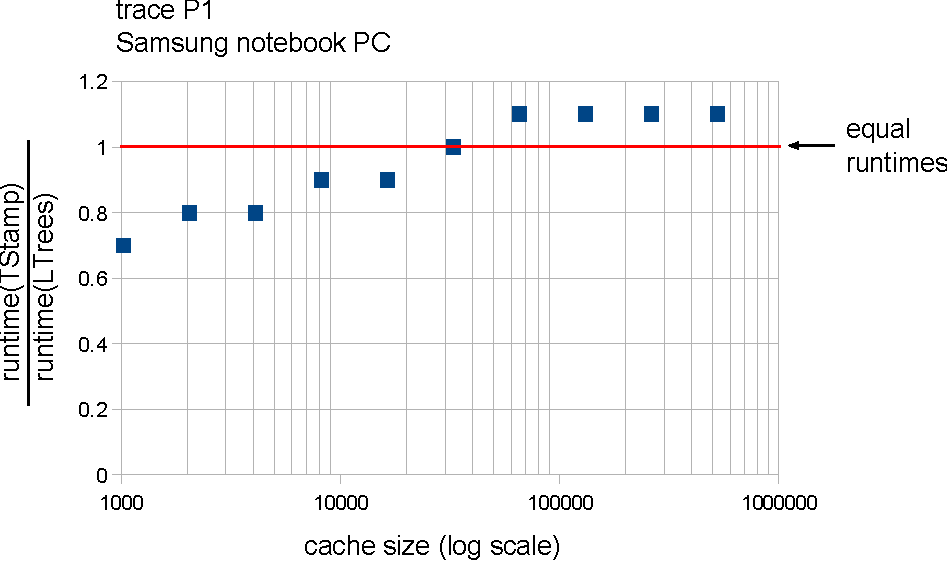
\includegraphics[scale=0.8]{./experiments/samsung_P1.pdf}
	\caption{The ratio runtime(TStamp)/runtime(LTrees) is plotted against the cache size.
                     The red line corresponds to points of equal runtimes.} 
	\label{fig:samsung_P1}
\end{figure}


% table ----------------------------------------------------------
\begin{table}[p]
\begin{center}
	trace P1 processed on Samsung notebook PC
	\begin{tabular}{|r||r|r|r|}
	  	\hline
                cache size                               &     runtime LTrees         &      runtime TStamp          &  runtime(TStamp)/ \\
                                                             &      (in seconds)            &      (in seconds)                 & runtime(LTrees)     \\
                \hline
                1024			             &             52                 &               36                     &            0.7            \\
		2048					     &     50                         &       38                             &    0.8                    \\								
		4096					     &     51                         &       39                             &    0.8                    \\	
		8192					     &     48                         &       41                             &    0.9                    \\	
		16384				     &     48                         &       43                             &    0.9                    \\	
		32768				     &     47                         &       46                             &    1.0                    \\	
		65536				     &     46                         &       50                             &    1.1                    \\	
		131072				     &     46                         &       51                             &    1.1                    \\	
		262144				     &     45                         &       49                             &    1.1                    \\	
		524288				     &     42                         &       45                             &    1.1                    \\
                \hline
	\end{tabular}
	\caption{Results for the trace P1 using the Samsung notebook PC.}
        \label{tab:samsung_P1}
\end{center}
\end{table}



%OOOOOOOOOOOOOOOOOOOOOOOOOOOOOOOOOOOOOOOOOOOOOOOOOOOOOOOOOOOOOOO
% plot  ----------------------------------------------------------
\begin{figure}[p]
	\centering
	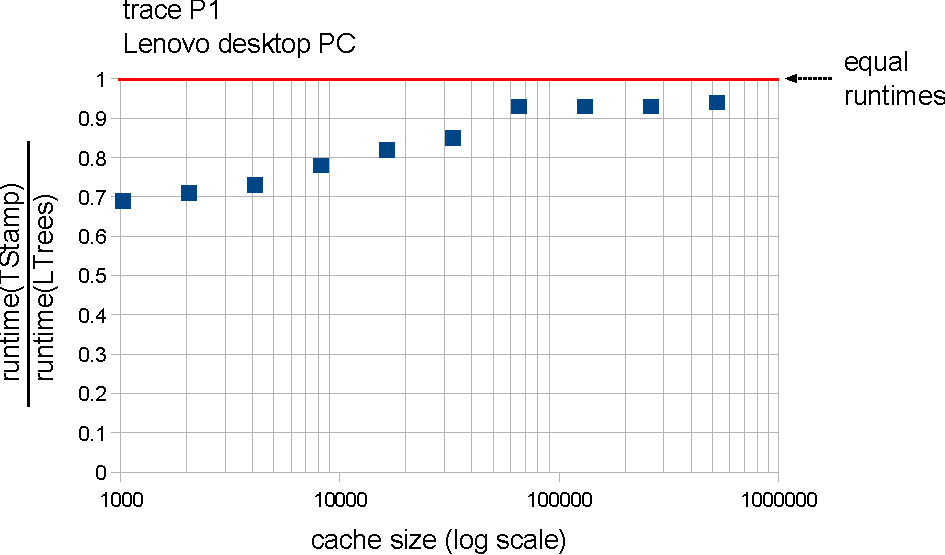
\includegraphics[scale=0.8]{./experiments/lenovo_P1.pdf}
	\caption{The ratio runtime(TStamp)/runtime(LTrees) is plotted against the cache size.
                     The red line corresponds to points of equal runtimes.} 
	\label{fig:lenovo_P1}
\end{figure}


% table ----------------------------------------------------------
\begin{table}[p]
\begin{center}
	trace P1 processed on Lenovo desktop PC
	\begin{tabular}{|r||r|r|r|}
	  	\hline
                cache size                               &     runtime LTrees         &      runtime TStamp          &  runtime(TStamp)/ \\
                                                             &      (in seconds)            &      (in seconds)                 & runtime(LTrees)     \\
                \hline
                1024			             &              5.336                &            3.667                        &          0.69              \\
		2048					     &      5.352                        &      3.792                              &    0.71                   \\								
		4096					     &      5.243                        &      3.808                              &     0.73                   \\	
		8192					     &      5.307                        &      4.135                              &     0.78                   \\	
		16384				     &      5.273                        &      4.306                              &     0.82                   \\	
		32768				     &      5.367                        &      4.556                              &     0.85                   \\	
		65536				     &      5.258                        &      4.868                              &     0.93                   \\	
		131072				     &      5.149                        &      4.769                              &     0.93                   \\	
		262144				     &      5.055                        &      4.697                              &     0.93                   \\	
		524288				     &      4.603                        &      4.338                              &     0.94                   \\
                \hline
	\end{tabular}
	\caption{Results for the trace P1 using the Lenovo desktop PC.}
        \label{tab:lenovo_P1}
\end{center}
\end{table}


%OOOOOOOOOOOOOOOOOOOOOOOOOOOOOOOOOOOOOOOOOOOOOOOOOOOOOOOOOOOOOOO
% plot  ----------------------------------------------------------
\begin{figure}[p]
	\centering
	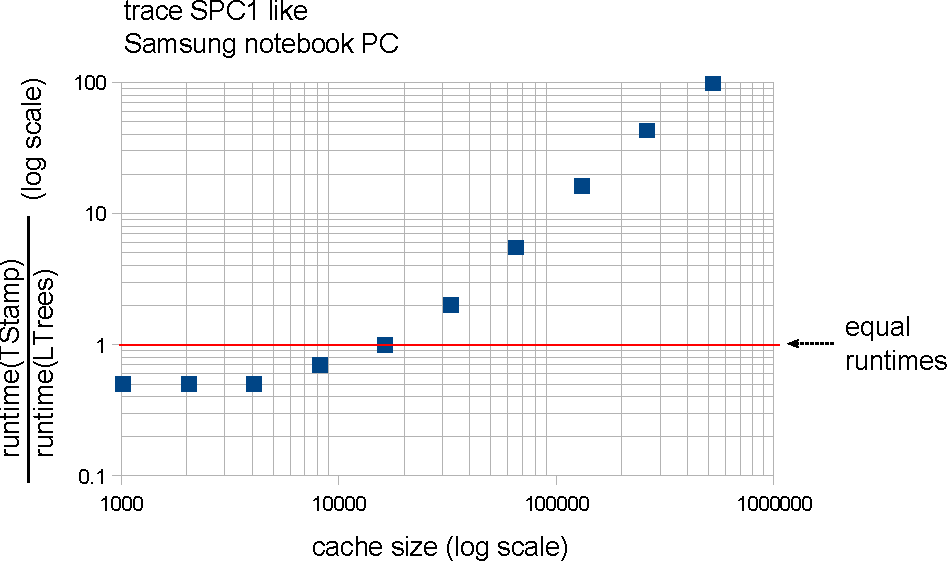
\includegraphics[scale=0.8]{./experiments/samsung_SPC1.pdf}
	\caption{The ratio runtime(TStamp)/runtime(LTrees) is plotted against the cache size.
                     The red line corresponds to points of equal runtimes.} 
	\label{fig:samsung_SPC1}
\end{figure}


% table ----------------------------------------------------------
\begin{table}[p]
\begin{center}
	trace SPC1 like processed on Samsung notebook PC
	\begin{tabular}{|r||r|r|r|}
	  	\hline
                cache size                               &     runtime LTrees         &      runtime TStamp          &  runtime(TStamp)/ \\
                                                             &      (in seconds)            &      (in seconds)                 & runtime(LTrees)     \\
                \hline
                1024			             &           139                   &                63                    &         0.5               \\
		2048					     &        141                      &        66                            &     0.5                   \\								
		4096					     &        138                      &        75                            &      0.5                  \\	
		8192					     &        137                      &        92                            &      0.7                  \\	
		16384				     &        138                      &       137                            &      1.0                  \\	
		32768				     &        137                      &       270                             &     2.0                   \\	
		65536				     &        139                      &       765                              &    5.5                    \\	
		131072				     &        144                      &       2313                             &     16.1                   \\	
		262144				     &        143                      &       6145                             &      43.0                  \\	
		524288				     &        145                      &      14212                              &      98.0                  \\
                \hline
	\end{tabular}
	\caption{Results for the trace SPC1 like using the Samsung notebook PC.}
        \label{tab:samsung_SPC1}
\end{center}
\end{table}



%OOOOOOOOOOOOOOOOOOOOOOOOOOOOOOOOOOOOOOOOOOOOOOOOOOOOOOOOOOOOOOO
% plot  ----------------------------------------------------------
\begin{figure}[p]
	\centering
	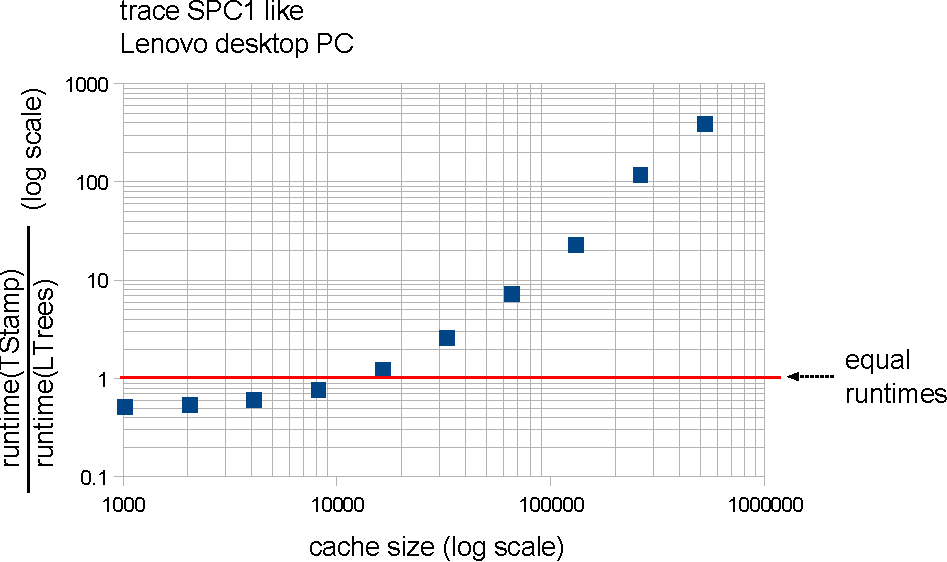
\includegraphics[scale=0.8]{./experiments/lenovo_SPC1.pdf}
	\caption{The ratio runtime(TStamp)/runtime(LTrees) is plotted against the cache size.
                     The red line corresponds to points of equal runtimes.} 
	\label{fig:lenovo_SPC1}
\end{figure}


% table ----------------------------------------------------------
\begin{table}[p]
\begin{center}
	trace SPC1 like processed on Lenovo desktop PC
	\begin{tabular}{|r||r|r|r|}
	  	\hline
                cache size                               &     runtime LTrees         &      runtime TStamp          &  runtime(TStamp)/ \\
                                                             &      (in seconds)            &      (in seconds)                 & runtime(LTrees)     \\
                \hline
                1024			             &          13.978                    &              7.084                      &     0.51                   \\
		2048					     &       14.071                       &      7.552                              &     0.54                   \\								
		4096					     &       14.056                       &      8.550                              &        0.61               \\	
		8192					     &       14.447                       &      11.108                              &     0.77                   \\	
		16384				     &       14.383                       &      17.597                              &     1.22                   \\	
		32768				     &       14.712                       &      38.282                              &     2.60                   \\	
		65536				     &       14.977                       &     108.904                               &    7.27                    \\	
		131072				     &       15.289                      &      348.368                              &     22.8                   \\	
		262144				     &       15.445                       &     1811.227                               &   117.2                     \\	
		524288				     &       15.929                       &     6365.187                               &   390.4                     \\
                \hline
	\end{tabular}
	\caption{Results for the trace SPC1 like using the Lenovo desktop PC.}
        \label{tab:lenovo_SPC1}
\end{center}
\end{table}


%OOOOOOOOOOOOOOOOOOOOOOOOOOOOOOOOOOOOOOOOOOOOOOOOOOOOOOOOOOOOOOO
% plot  ----------------------------------------------------------
\begin{figure}[p]
	\centering
	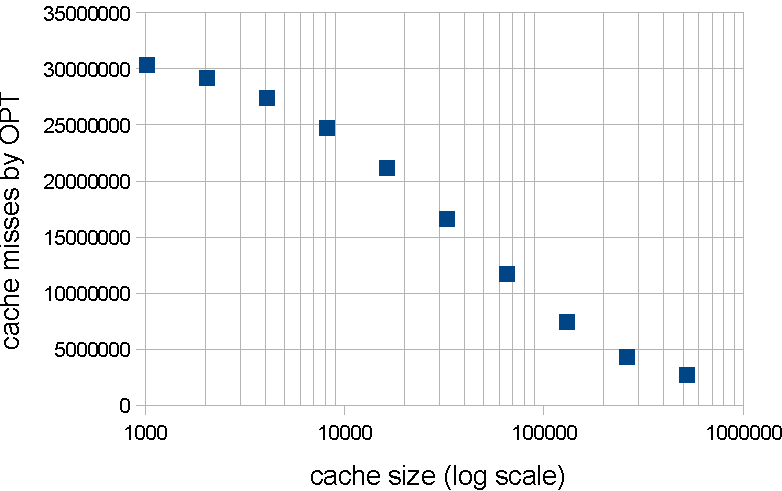
\includegraphics[scale=0.8]{./experiments/cacheMisses_P1.pdf}
	\caption{Cache misses caused by OPT when processing trace P1 for different cache sizes.} 
	\label{fig:cacheMisses_P1}
\end{figure}

% table ----------------------------------------------------------
\begin{table}[p]
%\begin{center}
	\centering
	\begin{tabular}{|r||r|r|r|r|}
	  	\hline
                cache size                               &    trace S1             &  trace P6         &      trace P1          &  trace SPC1 like   \\
                \hline
                1024			                    &      3,913,529           &       12,323,422   &   30,319,804    &   40,932,071 \\
		2048					     &     3,878,293           &      12,141,333   &    29,187,708    &   40,744,270 \\								
		4096					     &     3,828,086            &      11,799,023   &   27,381,737    &   40,480,354  \\	
		8192					     &     3,759,145           &       11,158,014   &   24,752,758    &   40,095,501  \\	
		16384				     &     3,658,723           &       9,940,268     &  21,182,902     &   39,512,083 \\	
		32768				     &     3,512,624           &       7,762,875    &   16,637,048     &    38,639,773 \\	
		65536				     &     3,270,542           &       4,196,139    &   11,741,790    &    37,353,435  \\	
		131072				     &     2,873,783           &       1,520,374    &   7,410,604      &    35,430,956 \\	
		262144				     &     2,297,465           &          827,165    &   4,293,906      &    32,562,546 \\	
		524288				     &     1,637,573           &          773,770    &   2,680,440      &    27,990,208 \\
                \hline
	\end{tabular}
	\caption{Number of cache misses caused by OPT when processing a trace at different cache sizes.
                     The values decrease with increasing cache size.}
        \label{tab:cacheMissesTraces}
%\end{center}
\end{table}


\newpage

\subsection{Discussion}
\textbf{Trace OLTP:} This is the smallest of the five examined traces. LTrees outperforms TStamp 
on all cache sizes. Starting at $k=1000$ LTrees is faster by a factor of 1.3, and this factor increases to 4.0
at $k=15000$.\\
\\
\textbf{Trace S1:} As expected the runtimes for LTrees are not influenced by the cache size $k$
since the amortized runtime per page request is $\oh(\alpha(2m))$ and thus independent of $k$.
In contrast, we observe that the times for TStamp strongly depend on the cache size. A larger $k$
also means a greater processing time because TStamp processes a page request in $O(k)$ time.

For smaller cache sizes (1024 to 4096) TStamp is faster by a factor of 2, but for greater 
cache sizes (131072 to 524288) LTrees  is faster by a factor of 10.\\
\\
\textbf{Trace P6:} Again the times for LTrees remain almost constant with increasing cache size (they
even decrease a little).
Surprisingly, TStamp is not affected by an increasing cache size. 
We can explain this by recalling that TStamp can still
be fast for large $k$ if the number of non-empty layers is small, see again remark (R1)
in section~\ref{sec:runtimeAnalysisTStamp}. This seems to be the case for this trace.
On all cache sizes TStamp outperforms LTrees.
For smaller $k$ TStamp is faster by a factor of 1.5. However, as $k$ increases this factor decreases 
to 1.1.
\\
\\
\textbf{Trace P1:} Here, the results are similar to P6. This suggests that P1 and P6 do not generate many
non-empty layers in the layer partition which is an advantage for TStamp.  \\
\\
\textbf{Trace SPC1 like:} The runtimes for LTrees increase by a negligible amount. 
By comparison the times for TStamp increase dramatically. For $k=1024$ TStamp is faster by a factor of 2.
However, for $k \geq 131072$ the situation is reversed and LTrees is 15 times faster (for $k=524288$ LTrees is even more than 100 times faster). \\
\\
\textbf{Number of cache misses:} In table~\ref{tab:cacheMissesTraces} we observe that the number
of cache misses caused by OPT decrease with increasing cache size $k$. The explanation is that a greater $k$ means 
a higher probability of finding a requested page in cache, which in turn implies a lower probability for a cache miss.  


%OOOOOOOOOOOOOOOOOOOOOOOOOOOOOOOOOOOOOOOOOOOOOOOOOOOOOOOOOOOOOOO
% plot  ----------------------------------------------------------
%\begin{figure}[p]
%	\centering
%	\includegraphics[scale=0.8]{./experiments/samsung_P6.pdf}
%	\caption{The ratio runtime(TStamp)/runtime(LTrees) is plotted against the cache size.
%                     The red line corresponds to points of equal runtimes.} 
%	\label{fig:samsung_P6}
%\end{figure}


% table ----------------------------------------------------------
%\begin{table}[p]
%\begin{center}
%	trace P6 processed on Samsung notebook PC
%	\begin{tabular}{|r||r|r|r|}
%	  	\hline
%                cache size                               &     runtime LTrees         &      runtime TStamp          &  runtime(TStamp)/ \\
%                                                             &      (in seconds)            &      (in seconds)                 & runtime(LTrees)     \\
%                \hline
%                1024			             &                              &                                    &                        \\
%		2048					     &                              &                                    &                        \\								
%		4096					     &                              &                                    &                        \\	
%		8192					     &                              &                                    &                        \\	
%		16384				     &                              &                                    &                        \\	
%		32768				     &                              &                                    &                        \\	
%		65536				     &                              &                                    &                        \\	
%		131072				     &                              &                                    &                        \\	
%		262144				     &                              &                                    &                        \\	
%		524288				     &                              &                                    &                        \\
%                \hline
%	\end{tabular}
%	\caption{Results for the trace P6 using the Samsung notebook PC.}
%        \label{tab:samsung_P6}
%\end{center}
%\end{table}




%----------------------------------------------------------------------------------------------------
\newpage
\section{Conclusion and future work}
\subsection{Conclusion}
For the traces SPC1 like and S1 TStamp is 2 times faster on smaller cache sizes, whereas for greater cache sizes
LTrees is more than 10 times faster. So, which data structure shall we choose to simulate the optimal 
offline paging algorithm OPT? A look at the absolute runtimes may give the answer, e.g. let us 
examine the times for the trace SPC1 like in table~\ref{tab:lenovo_SPC1}.

We measured the runtime for 10 different cache sizes ranging from $k=1024$ to $k=524288$. 
Due to its robustness LTrees required about 16 seconds for each $k$ which means that the overall runtime is 
$10 \cdot 16 \text{ seconds} = 160 \text{ seconds}$. TStamp on the other hand already requires 
more time with 350 seconds at $k=131072$, let alone for all 10 cache sizes together.
Thus, if we wish to simulate OPT for several cache sizes we should pick LTrees. 

Moreover, TStamp is only faster for smaller cache sizes where the runtime is small anyway, e.g. at 
$k=1024$ the difference between runtime(LTrees)=14 seconds and runtime(TStamp)=7 seconds
is 7 seconds. Compare this to $k=262144$ where runtime(LTrees)=16 seconds and 
runtime(TStamp)=1800 seconds = 30 minutes. Here, we have to wait for half an hour till TStamp
has processed the trace. 

For the trace P6 the results in figure~\ref{fig:lenovo_P6} and table~\ref{tab:lenovo_P6} are in favor of TStamp.
On all cache sizes TStamp outperforms LTrees. Trace OLTP demonstrates a reverse situation. 
Here, LTrees outperforms TStamp on all cache sizes. 

In summary, the robustness towards increasing cache sizes is a strong argument for selecting LTrees.
It means that when we conduct experiments we won't get surprised by a sudden increase of the runtime. 

\subsection{Future work}
For a future project or thesis it would be interesting to implement LTrees 
in C++ instead of Java. This rules out a possible influence of the Java garbage collector. 
Another aspect is the implementation of the nodes. For each node attribute we introduced 
an array, such as the parent array and the rank array. However, we could have also used
a \emph{Node class} that contains these attributes and whose objects represent the nodes. 
All nodes are then stored in an array 
of type \emph{Node}. We decided not to follow this approach in Java for two reasons. 
First, the objects require more space. Second, in Java there is no guarantee that the objects
are allocated contiguously~\cite{objectsContiguous_java}. In C++ the situation is different~\cite{objectsContiguous_cpp}, 
and it would be interesting to know if such an approach improves the runtime.

One could also examine how other path compression schemes and using union by size~\cite{galler64} 
instead of union by rank change the runtime. A survey of path compression schemes is 
given in~\cite{tarjan_leeuwen84, patwary10}. 

LTrees allows us to determine the empirical competitive ratio~\cite{moruz_soda12}. 
This could be used to decide adaptively which page replacement algorithm we should employ. 

Furthermore, LTrees can be utilized as a subroutine for the paging algorithm RLRU~\cite{boyar07} 
to improve the runtime from $\oh(\log(m))$ to $\oh(\alpha(2m))$ amortized time, where $m$ is 
the number of unique pages requested.

Moruz and Negoescu introduced the so-called attack rate $r$ which measures how ``hard'' a request sequence is~\cite{moruz_soda12}.
Due to its robustness towards different cache sizes it is possible for LTrees to determine $r$ in reasonable time. 

Finally, we want to mention the union-find data structure by Alstrup et al.~\cite{alstrup05} which supports
deletions in constant time, and which has been simplified by Ben-Amram and Yoffe~\cite{ben-amram11, ben-amram11_corrigendum}.
Using this data structure to implement the layer partition would make for a nice project.


\clearpage
\section*{Appendix}
\appendix
\addcontentsline{toc}{section}{Appendix}
\section{Interpretation of the layer partition}
We want to further describe the relationship between the layer partition $(\cl_0 | \cl_1 | ... | \cl_k)$ and the 
optimal offline paging algorithm OPT as done in~\cite{sea12_paper,moruz_soda12}.  When a page $p$ is requested it can be 
assigned to one of the following three categories:

\begin{enumerate}
 \item $p \in \cl_k$. Pages requested from $\cl_k$ have the property of being 
         in OPT's cache. For this reason they are called \emph{revealed}.

 \item $p \in \cl_0$. Pages requested from $\cl_0$ are not in OPT's cache and
         cause a page fault.

 \item $p \in \cl_i$ with $0<i<k$. These pages might be in OPT's cache, but this depends on the future requests.
         They are denoted \emph{unrevealed} since we cannot be sure that they are in OPT's cache.
\end{enumerate}

\noindent Let us revisit an example from section~\ref{sec:LayerPartition} with 
$M=\{1,2,3,4,5,6\}$ being the page-set, $k=3$ 
the cache size and $\sigma=(4,2,4,5,6,4,1,2,1,6,2,4)$ the request sequence.
The first $k=3$ pairwise distinct requested pages are $\{4,2,5\}$,  from which we can deduce the initial partition 
$(\cl_0 | \cl_1| \cl_2| \cl_3)=(1,3,6|\emptyset|\emptyset|4,2,5)$.
Now, according to our interpretation the pages in $\cl_k = \cl_3$ are in the cache of OPT. This 
is indeed the case since the first $k$ distinct pages will fill the initially empty cache (see figure~\ref{fig:layerPartition_Interpretation1a}). 


\begin{figure}[!htp]
	\begin{center}
	\includegraphics[scale=1.1]{./figures/layerPartition_Interpretation1a.pdf}
	\caption{Comparison of the layer partition with OPT's cache.} 
	\label{fig:layerPartition_Interpretation1a}
        \end{center}
\end{figure}

\newpage
\noindent Page 6 is requested next. Since 6 is in $\cl_0$ this causes a cache miss and we will have to evict one of 
the pages 4,2,5 from the cache. The layer partition translates this by shifting 4,2,5 from $\cl_k$ to $\cl_{k-1}$ such that 
 pages 4,2,5 become unrevealed. For these pages we cannot be sure anymore that they are in OPT's cache since one of them
gets replaced (see figure~\ref{fig:layerPartition_Interpretation1b}).

\begin{figure}[!htp]
	\begin{center}
	\includegraphics[scale=1.1]{./figures/layerPartition_Interpretation1b.pdf}
	\caption{Comparison of the layer partition with OPT's cache.} 
	\label{fig:layerPartition_Interpretation1b}
        \end{center}
\end{figure}


\newpage
% Bibliography--------------------------------------------------------------------------------------
\begin{thebibliography}{99}

	\bibitem{belady66_opt}
	Belady, L. A. A study of replacement algorithms for virtual storage computers. 
        \emph{IBM Systems Journal}, 5(1966):78-101. 
	
	\bibitem{boyar07}
	J. Boyar, L. M. Favrholdt, and K. S. Larsen. The relative worst-order ratio applied
	to paging. \emph{Journal of Computer and System Sciences}, 73(5):818-843, 2007.

	\bibitem{brodal11}
	Gerth St\o lting Brodal, Gabriel Moruz, Andrei Negoescu: OnlineMin: A Fast Strongly Competitive Randomized Paging Algorithm. 
        \emph{WAOA 2011}: 164-175

        \bibitem{memory_hierarchy}
	There are actually more levels in the memory hierarchy: CPU, L1 cache, L2 cache, RAM, hard disk.
        Instead of RAM and hard disk one can also examine the relationship between two other levels such as
	L2 cache and RAM,
        see \emph{Memory Hierarchy Design - Part 1. Basics of Memory Hierarchies} by  
	John L. Hennessy, Stanford University, and David A. Patterson, University of California, Berkeley - September 25, 2012.
	\url{http://www.edn.com/design/systems-design/4397051/Memory-Hierarchy-Design-part-1}	

	\bibitem{albers99_brics}
          Susanne Albers. Lecture notes on Competitive Online Algorithms. 
          \emph{BRICS, Aarhus university}, 1996.  
          \url{http://www2.informatik.hu-berlin.de/~albers/papers/brics.pdf}
  
	\bibitem{johncctang} % youtube videos demonstrating paging algorithms
	  \url{http://www.youtube.com/user/johncctang}.

	\bibitem{moruz_soda12}
        Gabriel Moruz, Andrei Negoescu. Outperforming LRU via competitive analysis on parametrized inputs for paging. \emph{SODA 2012}: 1669-1680

	\bibitem{albers03_survey}
        Susanne Albers. Online algorithms: a survey. \emph{Math. Program.}, 97(1-2): 3-26 (2003)

	\bibitem{sleator85}  % LRU is k-competitive
         Daniel Dominic Sleator and Robert Endre Tarjan. Amortized Efficiency of List Update and Paging Rules.
         \emph{Communications of the ACM}, 28:202-208, 1985. \url{http://www.cs.cmu.edu/~sleator/papers/amortized-efficiency.pdf}

	\bibitem{chrobak99} %LRU is better than FIFO
         M. Chrobak, J. Noga. LRU is better than FIFO. \emph{Algorithmica}, 23:180-185, 1999.

	\bibitem{koutsoupias00} % layer partition
	E. Koutsoupias and C. H. Papadimitriou. Beyond competitive analysis. \emph{SIAM
	Journal on Computing}, 30:300-317, 2000.

	\bibitem{sea12_paper}
        G.Moruz, A. Negoescu, C. Neumann, and V.Weichert. Engineering efficient paging
        algorithms. In \emph{Proc. 11th International Symposium on Experimental Algorithms},
        2012. 

	\bibitem{galler64} % galler fischer data structure
	  B. A. Galler and M. J. Fischer. An improved equivalence algorithm. 
	  \textit{Communications of the ACM}, 7(5):301-303, 1964.
	
	\bibitem{tarjan75}  % union by rank
	  R. E. Tarjan. Efficiency of a good but not linear set union algorithm. 
	  \textit{Journal of the ACM}, 22(2):215-225, 1975.  
	  
	\bibitem{tarjan_golumbic}
	  M. C. Golumbic and I. B.-A. Hartman. \emph{Graph Theory, Combinatorics and Algorithms:
	Interdisciplinary Applications (Operations Research/Computer Science
	Interfaces Series)}. Springer-Verlag New York, Inc., 2005.
	
	\bibitem{tarjan83}
	  R. E. Tarjan. \emph{Data structures and network algorithms}. Society for Industrial and
    Applied Mathematics, 1983.
  
	\bibitem{inverse_ackermannFunction}
        We use the one-parameter version $\alpha(n)$ of the inverse Ackermann function, but in his original work
        Tarjan uses the two parameter version $\alpha(m,n)$~\cite{tarjan83,tarjan75}. The relationship between them is described by Jeff 
        Erickson in his lecture notes~\cite{jeffe}. Cormen et al. also use the one-parameter version in their book~\cite{cormen_CLRS}.
	Tarjan himself describes his result with the one-parameter version in~\cite{tarjan_golumbic}.   
        Moreover, Tarjan does not necessarily perform $n$ makeset operations in the beginning to create $n$ elements. 
        He considers $n$ makeset, at most $n-1$ union and $m \geq n$ find operations in an arbitrary order.
	
	\bibitem{jeffe}
         Jeff Erickson. Algorithms Course Materials,
        Chapter 16: Data Structures for Disjoint Sets,  
	Department of Computer Science, University of Illinois at Urbana-Champaign, 2011.
        \url{http://www.cs.uiuc.edu/~jeffe/teaching/algorithms/}

	\bibitem{cormen_CLRS}
        Thomas H. Cormen, Charles E. Leiserson, Ronald L. Rivest, Clifford Stein: Introduction to Algorithms (3. ed.). MIT Press 2009.

	\bibitem{gallerFischer_javaApplet}
        \url{http://www.cs.unm.edu/~rlpm/499/uf.html}

	\bibitem{brPreiss_onlineBook}
	Bruno R. Preiss. \emph{Data Structures and Algorithms with Object-Oriented Design Patterns in Java}.
	\url{http://www.brpreiss.com/books/opus5/html/page410.html}

	\bibitem{LTrees_find_index_i}
	We can determine the index $i$ for a page $p \in \cl_i$ with $0<i<k$ as follows:
        we first apply a find($p$) operation which returns the root node $r$ in $\oh(\alpha(2m))$ time.
	From $r$ we follow the left pointers and count the number of layers we traverse (including the empty layers) until we reach the root node of $\cl_0$,
	which requires $\oh(k)$ time. This gives us the value for $i$ in $\oh( \alpha(2m) + k)$ time.
	If the number of non-empty layers is $l<k$, then the time reduces to $\oh( \alpha(2m) + l)$.
       
       \bibitem{andrei_idea}
    	My advisor Andrei Negoescu had the idea of removing elements in a tree by using lazy deletion.
	He also devised the steps of the cleanup procedure.
  
	\bibitem{arc_paper}
	Nimrod Megiddo and Dharmendra S. Modha. ARC: A Self-Tuning, Low Overhead Replacement Cache. 
        In \emph{USENIX Conference on File and Storage Technologies (FAST 03)}, San Francisco, CA, pp. 115-130, March 31-April 2, 2003. 
	\url{http://www.almaden.ibm.com/cs/people/dmodha/}
	
	\bibitem{queue_stackoverflow}
        \url{http://stackoverflow.com/questions/2313062/a-fast-queue-in-java}

	\bibitem{queue_primitive}
        \url{http://harvestsoft.net/files/queue.pdf}

	\bibitem{objectsContiguous_java}
        \url{http://stackoverflow.com/questions/9632288/can-i-allocate-objects-contiguously-in-java}

	\bibitem{objectsContiguous_cpp}
        \url{http://stackoverflow.com/questions/8297993/how-is-an-array-of-objects-stored-in-memory}

	\bibitem{tarjan_leeuwen84}
	R. Tarjan and J. van Leeuwen. Worst-case analysis of set union algorithms. \emph{Journal of the ACM (JACM)}, Volume 31 Issue 2, 1984.

	\bibitem{patwary10}
        Md. Mostofa Ali Patwary, Jean Blair and Fredrik Manne. Experiments on Union-Find Algorithms for the Disjoint-Set Data Structure. 
        \emph{Proceedings of 9th International Symposium on Experimental Algorithms (SEA'10)}, Springer LNCS 6049, pp. 411-423, 2010.

	\bibitem{alstrup05}
        Stephen Alstrup, Inge Li G\o rtz, Theis Rauhe, Mikkel Thorup, Uri Zwick. Union-Find with Constant Time Deletions. \emph{ICALP 2005}: 78-89

	\bibitem{ben-amram11}
	Amir M. Ben-Amram, Simon Yoffe: A simple and efficient Union-Find-Delete algorithm. \emph{Theor. Comput. Sci.}, 412(4-5): 487-492, 2011.

	\bibitem{ben-amram11_corrigendum}
        Amir M. Ben-Amram, Simon Yoffe: Corrigendum to "A simple and efficient Union-Find-Delete algorithm" [Theoret. Comput. Sci. 412(4-5) 487-492]. 
        \emph{Theor. Comput. Sci.}, 423: 75, 2012.

\end{thebibliography}

\end{document}

